%%%%%%%%%%%%%%%%%%%%%%%%%%%%%%%%%%%%%%%%%%%%%%%%%%%%%%%%%%%%%%%%%%%%%%%%%%%%%%%%
%2345678901234567890123456789012345678901234567890123456789012345678901234567890
%        1         2         3         4         5         6         7         8

\documentclass[letterpaper, 10 pt, conference]{ieeeconf}  % Comment this line out
                                                          % if you need a4paper
%\documentclass[a4paper, 10pt, conference]{ieeeconf}      % Use this line for a4
                                                          % paper

\IEEEoverridecommandlockouts                              % This command is only
                                                          % needed if you want to
                                                          % use the \thanks command
\overrideIEEEmargins
% See the \addtolength command later in the file to balance the column lengths
% on the last page of the document

\usepackage{graphicx}
\usepackage{graphics}
\usepackage{amsmath}
\usepackage{float}

\title{\LARGE \bf
Informe de Trabajo Integrador Final IPyAN
}

\author{Tomás Vidal\\ %\vspace{1cm}
{\it Introducci\'on a la Programaci\'on y An\'alisis Num\'erico, Depto. de Ciencias B\'asicas}\\  {\it Facultad de Ingenier\'ia, UNLP, La Plata, Argentina.}}                                            % <-this % stops a space

\begin{document}

\maketitle
\thispagestyle{empty}
\pagestyle{empty}

%%%%%%%%%%%%%%%%%%%%%%%%%%%%%%%%%%%%%%%%%%%%%%%%%%%%%%%%%%%%%%%%%%%%%%%%%%%%%%%%
\begin{abstract}

    A continuaci\'on se detalla como se encuentran los valores del capacitor, inductor y resistencia, adem\'as del valor $u_{s}(t)$ del circuito el\'ectrico presente en Fig. 1. La principal aplicaci\'on de este circuito es atenuar las frecuencias bajas de la señal que se le entregue, por eso adem\'as de estudiar los valores de sus componentes se interioriza en el estudio de la señal de salida $u_{s}(t)$ con respecto de diferentes tipos de señales sinusoidales.
    Para poder aproximar $u_{s}(t)$ se hace uso de los m\'etodos num\'ericos de polinomios de Lagrange y m\'inimos cuadrados, y se espera que tenga una forma exponencial decreciente, y luego de aplicar los m\'etodos se concluye que efectivamente la tensi\'on analizada tiene este comportamiento y que para aproximar los datos que no tienen error es mejor interpolarlos, al contrario de los que se sabe que tienen error, pues a estos \'ultimos es mejor hacerles un ajuste (exponencial en este caso).
    Posterior a \'esto se aproxima el valor de la resistencia haciendo un ajuste de los datos, y despejando de relaciones f\'isicas conocidas, finalmente se obtienen errores relativos del 5.50\% y 0.05\% tomando ventaja de la precisi\'on en diferentes intervalos de tiempo. Los valores del capacitor y inductor se hayan a partir de las ecuaciones f\'isicas que describen sus comportamientos en los circuitos el\'ectricosy, en estos casos se llega a las aproximaciones a partir del m\'etodo num\'erico de Simpson 3/8, pues con 200 puntos de mediciones se tiene un error relativo de 6.46\% (L) y 5.75\% (C).
    Para analizar la salida con respecto a las diferentes sinusoides en la entrada se hace uso de los m\'etodos de Euler, Taylor de orden 2, Adams Bashforth y Runge Kutta 4, concluyendo que el m\'etodo num\'erico m\'as efectivo es Taylor de orden 2 y que Runge Kutta 4 no converge para todas las frecuencias estudiadas. Tambi\'en se encuentra que el circuito atenua las frecuencias bajas en la salida a partir de 200hz.

\end{abstract}


%%%%%%%%%%%%%%%%%%%%%%%%%%%%%%%%%%%%%%%%%%%%%%%%%%%%%%%%%%%%%%%%%%%%%%%%%%%%%%%%
\section{INTRODUCCCI\'ON}

    En este informe se describen las metodolog\'ias implementadas y los resultados que se obtuvieron con sus significados referentes a los problemas que se pretenden responder y, que est\'an en el Trabajo Pr\'actico Integrador 2020.
    Todos los problemas tienen su respetivo archivo .m donde se encuentra el c\'odigo en matlab/octave para resolver num\'ericamente el problema en concreto, los mismos se encuentran adjuntos al informe, adem\'as de resultados num\'ericos archivados, aunque el lector puede tomarse la libertad de correr los c\'odigos y comprobar los mismos.
    Para poder comenzar a estudiar y calcular el valor aproximado de $u_{s}(t)$ primero se debi\'o realizar un an\'alisis del circuito con el objetivo de conocer aproximadamente el resultado esperado; al hacer esto se puede observar que $u_{s}(t)$ tendr\'a un comportamiento exponencial decreciente, pues el voltage provisto por la fuente $u_{e}$ se ver\'a disminuido progresivamente con la carga del capacitor, hasta que \'este se cargue por completo anulando el voltage en $u_{s}(t)$, dado que se conoce que la carga de un capacitor es exponencial se espera que la salida tenga el efecto inverso, es decir, una exponencial decreciente y adem\'as se deduce:

    \[ u_{s}(t) = u_{e} - u_{c}(t) \]

    Despu\'es de haber analizado \'esto se puede proseguir a implementar las resoluciones num\'ericas.

    \begin{figure}[H]
    \centering
    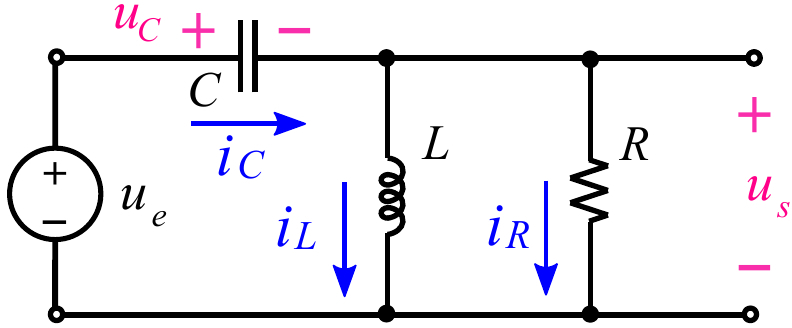
\includegraphics[width=0.43\textwidth]{./circuito.jpg}
    \caption{}
    \label{fig:fig}
    \end{figure}

\section{M\'etodos Implementados}

    En esta secci\'on se desarrollan los m\'etodos num\'ericos implementados a lo largo del informe. Los mismos fueron desarrollados matem\'aticamente como se los aplic\'o en el c\'odio para que sean facilmente implementables en cualquier lenguage de programaci\'ion.

\subsection{Lagrange}

El m\'etodo de Lagrange [1] implica obtener una funci\'on polinomial de grado N ($P_N(x)$) que tiene la forma:
\[ P_N(x) = \sum_{n=0}^{N}L_{n,N}(x)f(x_n) \]
\[ L_{n,N}(x_{i}) = \begin{cases} 1, x_{i} = x_{n} \\ 0, x_{l} \neq x_{n} \\  \end{cases} \]
con $ n,l = 0,1,\cdots,N $
Esto permite que en cada $x_{l}$ el polinomio coincida con el valor del punto dado.

\subsection{M\'inimos cuadrados}

Teniendo $f(x) = a_{0} + a_{1}x$ se aproxima $a_{0}$ y $a_{1}$ con el m\'etodo, haciendo uso de las ecuaciones:

\[ a_{0} = \frac{\sum_{i=1}^{m}x_{i}^{2}\sum_{i=1}^{m}f(x_{i})-\sum_{i=1}^{m}x_{i}f(x_{i})\sum_{i=1}^{m}x_{i}}{m(\sum_{i=1}^{m}x_{i}^{2})-(\sum_{i=1}^{m}x_{i})^{2}} \]
\[ a_{1} = \frac{\sum_{i=1}^{m}x_{i}f(x_{i})-\sum_{i=1}^{m}x_{i}\sum_{i=1}^{m}f(x_{i})}{m(\sum_{i=1}^{m}x_{i}^{2})-(\sum_{i=1}^{m}x_{i})^{2}} \]

\subsection{Simpson 3/8}

Sea la integral
\[ I = \int_{a}^{b}f(x) \]
Se obtiene una aproximaci\'on de la misma con:

\[ I \approx \frac{3h}{8}[f(x_{0}) + 3\sum_{i=1}^{N/3}(f(x_{3i-2} + f(x_{3i-1})) + \]
\[ 2\sum_{i=1}^{N/3-1}(f(x_{3i}) + f(x_{N}))] \]


\subsection{Euler}
   
Todos los sistemas de ecuaciones que se resuelven con estos m\'etodos requieren que cada ecuaci\'on sea aproximada con el valor en\'esimo antes de seguir la proxima iteracion (es decir n+1); entonces si se tiene el siguiente sistema de ecuaciones:

\[ \begin{cases} y'_1 = y_2 = f1(x, y_1, y_2) \\ y'_2 = - \frac{1}{RC} y_2 - \frac{1}{LC} y_1 = f_2(x, y_1, y_2) \end{cases} \]

Aplicando el m\'etodo $y_1$ e $y_2$ se pueden aproximar con:

\[ \begin{cases} y_1(x_{n+1}) = y_1(x_n) + hy_2(x_n) \\ y_2(x_{n+1}) = y_2(x_n) + hf_2(x_n, y_1(x_n), y2(x_n)) \end{cases} \]

Donde h es el paso de iteraci\'on.
Este m\'etodo tiene un error global $O(h)$.

\subsection{Taylor orden 2}

Para poder aplicar este m\'etodo se requiere una derivada m\'as de la que se tiene en el problema original, por lo tanto se debi\'o encontrar de la siguiente forma:

\[ \frac{ \partial^2 {u_{S}(t)}}{\partial t^2} = - \frac{1}{RC}\frac{\partial{u_{S}(t)}}{\partial{t}} - \frac{u_{S}(t)}{LC} + \frac{\partial^2{u_{e}(t)}}{{\partial{t^2}}} \]

\[ \frac{ \partial^3 {u_{S}(t)}}{\partial t^3} = - \frac{1}{RC}\frac{\partial^2{u_{S}(t)}}{\partial{t^2}} - \frac{\partial{u_{S}(t)}}{\partial{tLC}} + \frac{\partial^3{u_{e}(t)}}{{\partial{t^3}}} \]

Primero se despeja la m\'axima derivada, y luego se deriva en ambos lados de la ecuaci\'on y as\'i se tiene la derivada que se requiere. Luego se prosigue al igual que con el m\'etodo de Euler, a exepci\'on de que ahora se agrega un nuevo t\'ermino en ambas ecuaciones:

\[ \begin{cases} y_1(x_{n+1}) = y_1(x_n) + hy_2(x_n) + \frac{h^2}{2!}f(x_n, y_1, y_2) \\ y_2(x_{n+1}) = y_2(x_n) + hf(x_n, y_1(x_n), y2(x_n)) + \\
+ \frac{h^2}{2!}f_2(x_n, y_1, y_2) \end{cases} \]

Donde $f_2$ es la derivada que se acaba de encontrar, esta depende de $x$, $y_1$ e $y_2$ porque se deben reemplazar las variables acorde al sistema de ecuaciones planteado.

Este m\'etodo tiene un error global $O(h^2)$.

\subsection{Adams Bashforth orden 3}

Para este m\'etodo se requiere tener al menos 3 puntos iniciales, \'estos se obtuvieron del m\'etodo de Taylor y de la soluci\'on anal\'itica; para la aproximaci\'on se utiliz\'o el siguiente sistema de ecuaciones:

\[ \begin{cases} y_1(x_{n+1}) = y_1(x_n) + \frac{h}{12}[23f_1(x_n, y_1(x_n), y_2(x_n)) - \\ 16f_1(x_{n-1}, y_1(x_{n-1}), y_2(x_{n-1})) \\ + 5f_1(x_{n-2}, y_1(x_{n-2}), y_2(x_{n-2}))] \\ y_2(x_{n+1}) = y_2(x_n) + \frac{h}{12}[23f_2(x_n, y_1(x_n), y_2(x_n)) - \\ 16f_2(x_{n-1}, y_1(x_{n-1}), y_2(x_{n-1})) \\ + 5f_2(x_{n-2}, y_1(x_{n-2}), y_2(x_{n-2}))] \end{cases} \]

Este m\'etodo tiene un error global $O(h^3)$

\subsection{Runge Kutta 4}

Para resolver la ecuaci\'on diferencial con \'este m\'etodo se aproxim\'o con:

\[ \begin{cases} 
    k11 = hf1(x_n, y_1(x_n), y_2(x_n)) \\
    k12 = hf2(x_n, y_1(x_n), y_2(x_n)) \\
    k21 = hf1(x_n, \frac{h}{2} + y_1(x_n), \frac{1}{2}k11 + y_2(x_n)) \\
    k22 = hf2(x_n, \frac{h}{2} + y_1(x_n), \frac{1}{2}k12 + y_2(x_n)) \\
    k31 = hf1(x_n, \frac{h}{2} + y_1(x_n), \frac{1}{2}k21 + y_2(x_n)) \\
    k32 = hf2(x_n, \frac{h}{2} + y_1(x_n), \frac{1}{2}k22 + y_2(x_n)) \\
    k41 = hf1(x_n, \frac{h}{2} + y_1(x_n), k31 + y_2(x_n)) \\
    k42 = hf2(x_n, \frac{h}{2} + y_1(x_n), k32 + y_2(x_n)) \\
    y_1(x_{n+1}) = y_1(x_n) + \frac{1}{6}[k11 + 2k21 + 2k31 + k41] \\
    y_2(x_{n+1}) = y_2(x_n) + \frac{1}{6}[k12 + 2k22 + 2k32 + k42]

\end{cases} \]

    Donde $f1$ y $f2$ ya se definieron previamente. Este m\'etodo tiene un error global $O(h^4)$.

\section{Ejercicio 1}

\subsection{MARCO TE\'ORICO}

    Para el caso del an\'alisis de $u_{s}(t)$ se aplic\'o el m\'etodo de Lagrange. Este m\'etodo es considerado apto para el ejercicio 1 a y b, pues en estos casos sabemos que los valores tomados son exactos, entonces la funci\'on que los contiene debe interpolarlos.
    Para ambos incisos se utiliz\'o el mayor orden polinomial posible, pues de otra forma se introduc\'ia mucho error en los extremos del intervalo debido a los efectos de estos polinomios (con un total de 25 muestras en el a y 50 en el b). 

    \begin{figure}[H]
    \centering
    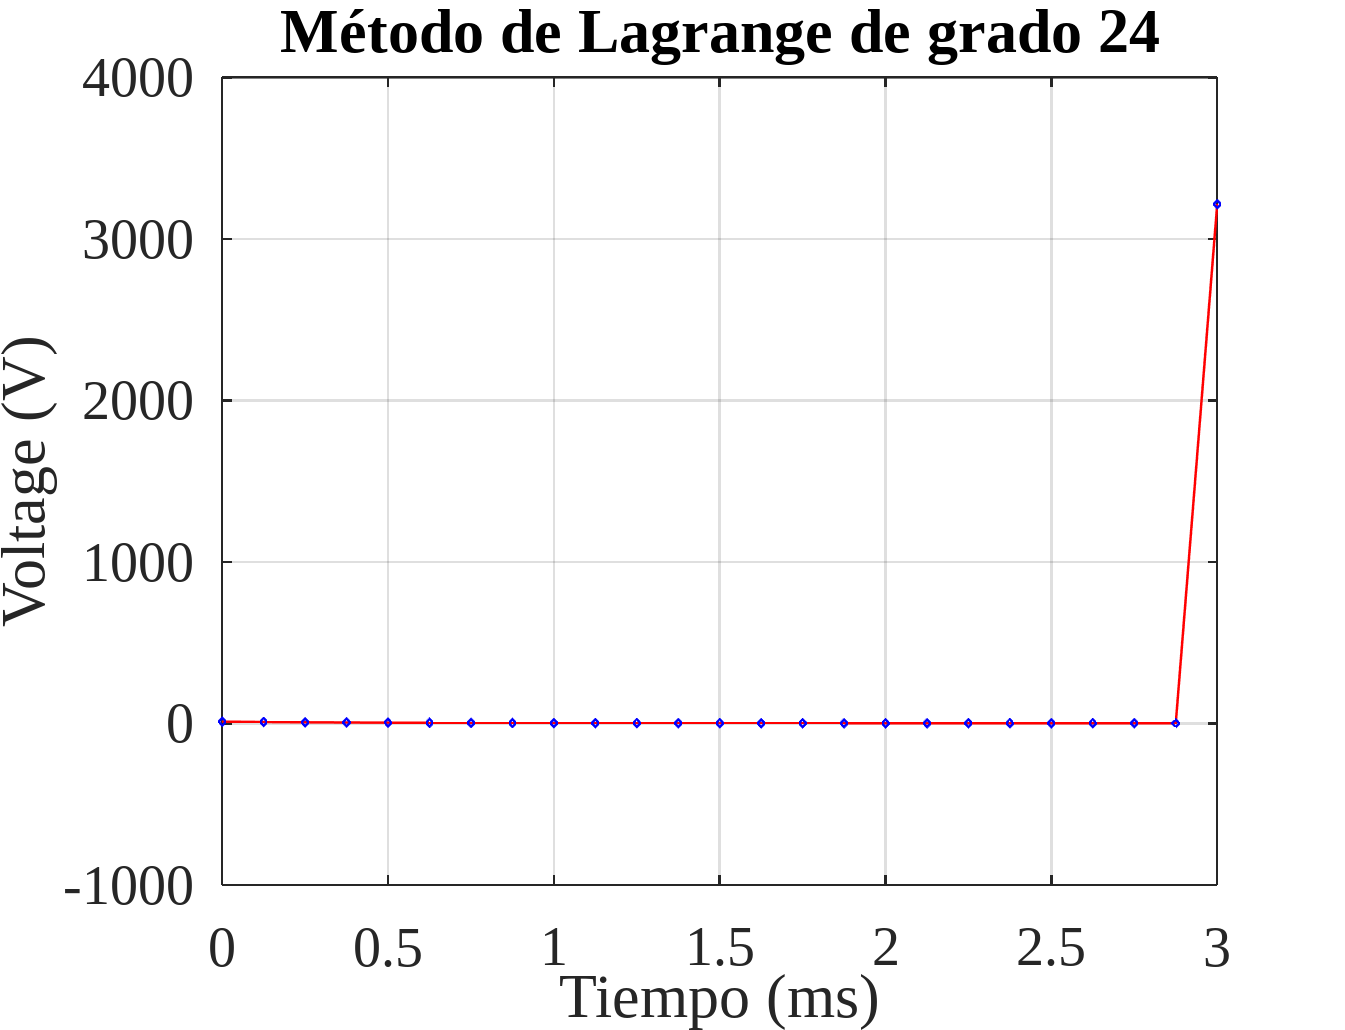
\includegraphics[width=0.43\textwidth]{./../plots/ej1/ej1-a-con-error.png}
    %\caption{}
    \label{fig:fig}
    \end{figure}

    \begin{figure}[H]
    \centering
    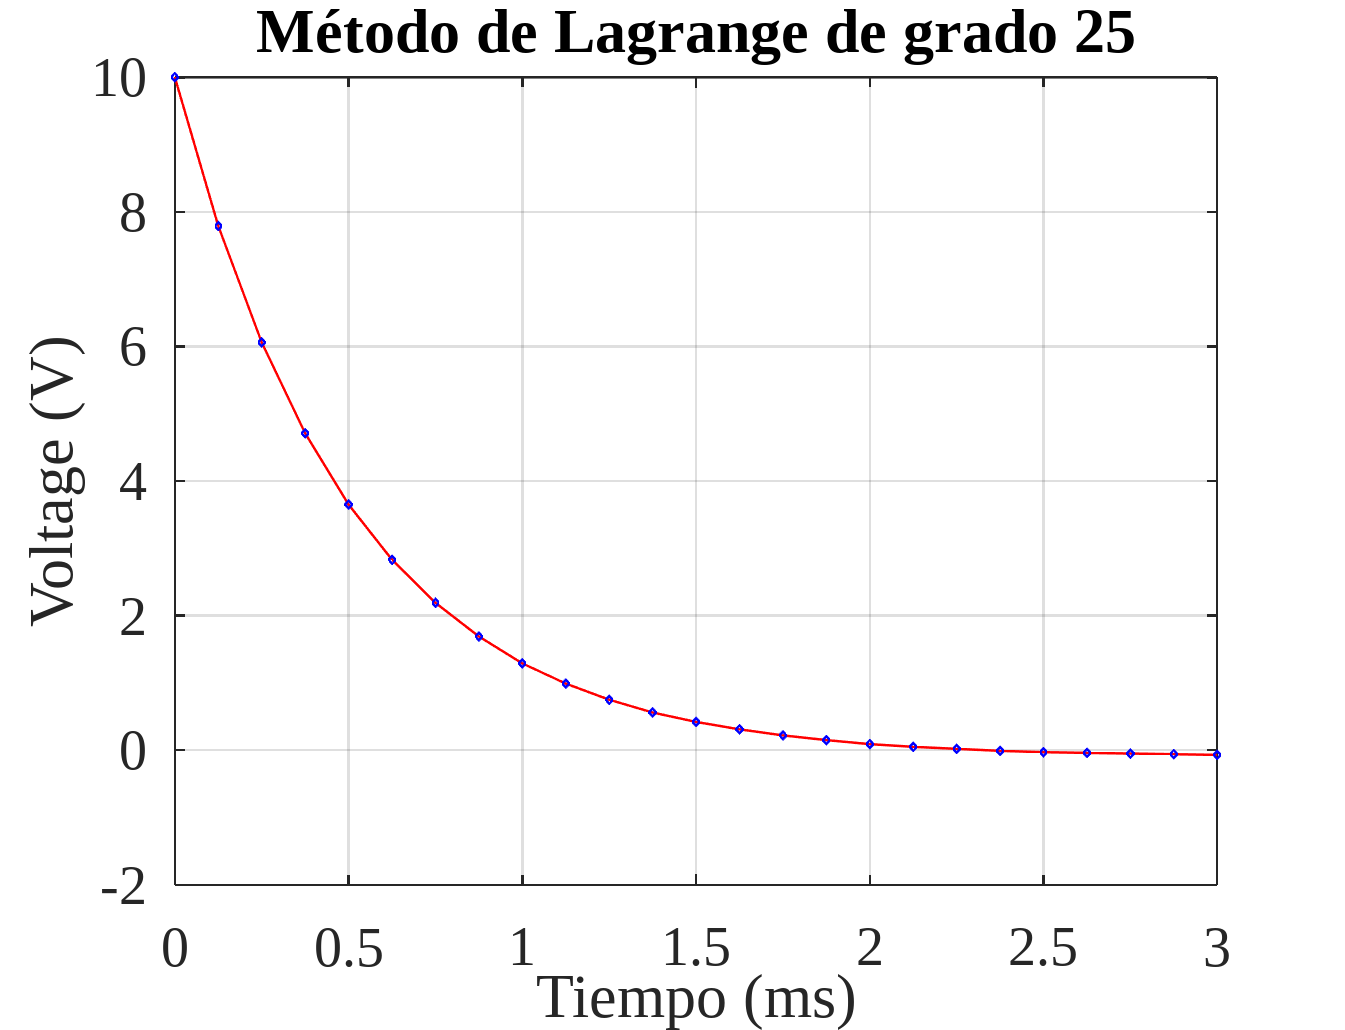
\includegraphics[width=0.43\textwidth]{./../plots/ej1/ej1-a.png}
    %\caption{}
    \label{fig:fig}
    \end{figure}

    \begin{figure}[H]
    \centering
    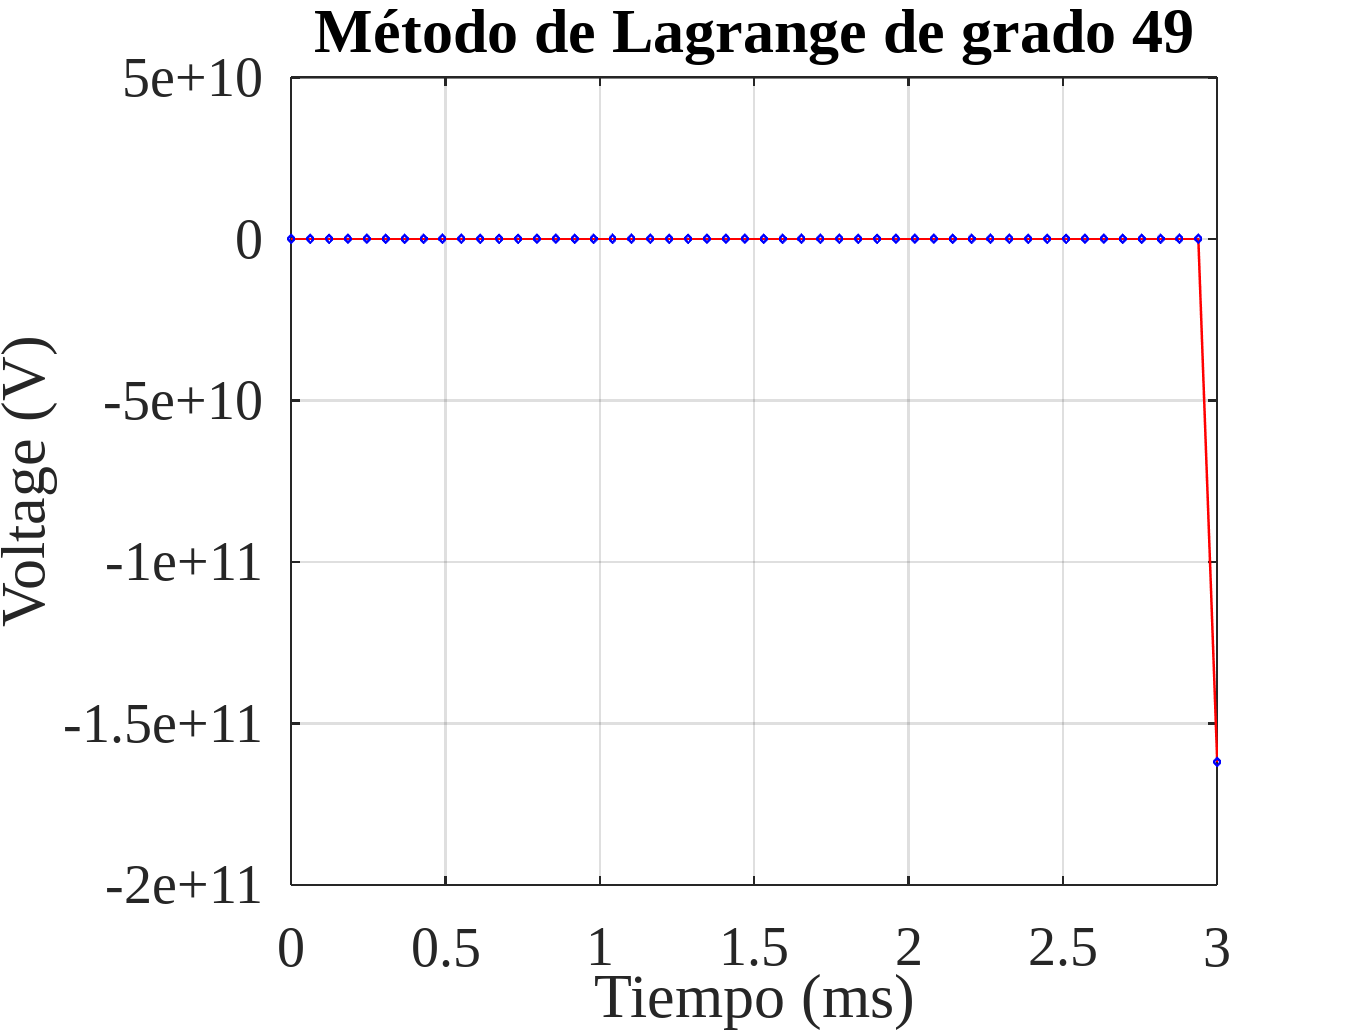
\includegraphics[width=0.43\textwidth]{./../plots/ej1/ej1-con-error.png}
    %\caption{}
    \label{fig:fig}
    \end{figure}

    \begin{figure}[H]
    \centering
    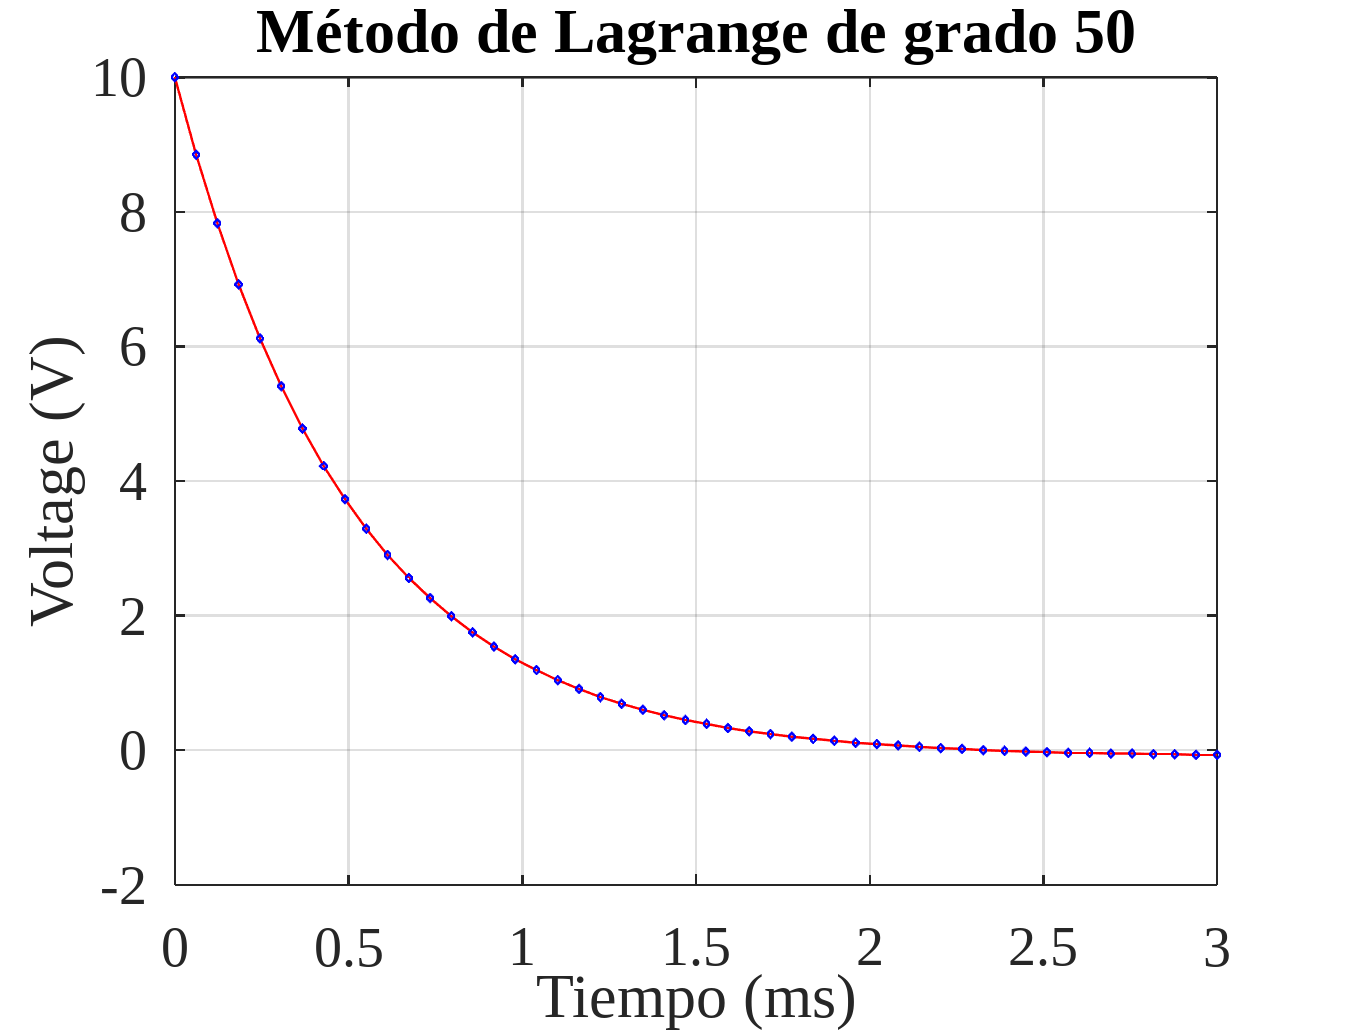
\includegraphics[width=0.43\textwidth]{./../plots/ej1/ej1-b.png}
    %\caption{}
    \label{fig:fig}
    \end{figure}

    En el caso del inciso C se aplic\'o el m\'etodo de m\'inimos cuadrados, pues los datos tienen error, (es decir que no se sabe si la funci\'on realmente los interpola) se sabe que la funci\'on tiene una forma exponencial:

    \[ f(x) = BA^x = Y \] 

    Por lo que para poder aplicar el m\'etodo se deben linealizar los par\'ametros A y B, aplicando logaritmo natural se tiene: 

    \[  Ln(Y) = Ln(BA^x) \] 

    Aplicando propiedades del logaritmo:

    \[ Ln(Y) = Ln(B) + Ln(A)x \]

    Reescribiendo:

    \[ \bar{Y} = \bar{B} + \bar{A}x \]

    Ahora si se puede aplicar el m\'etodo de m\'inimos cuadrados; es importante destacar que no estamos hayando el valor de $B$ directamente, sino que estamos buscando $\bar{B} \approx B$, y adem\'as usamos $\bar{Y} \approx Y$, por lo que \'esto introduce un nuevo error adem\'as del presente por el m\'etodo, que se debe tener en cuenta si se quiere lograr mayor precisi\'on.
    Entonces para obtener una aproximaci\'on de $A$ se debe aplicar exponencial:

    \[ A \approx e^{\bar{A}} \]

    Y con \'esto ya se tienen los par\'ametros necesarios para construir la funci\'on que ajusta exponencialmente los datos:

    \[ Y \approx Bx^{A} \]

    \subsection{C\'odigo matlab/octave}

    La dificultad para aplicar el m\'etodo de m\'inimos cuadrados se encuentra cuando hay puntos que tienen valores negativos o cero, pues hay aplicar el logaritmo para linealizar la ecuaci\'on y estos datos se salen del dominio del logaritmo, por eso para solventar este problema se aplic\'o una traslaci\'on a la variable dependiente de 6.65 unidades, ya que despu\'es probar distintos valores de traslaci\'on se comprob\'o que este \'ultima introduc\'ia menos error; y al primer valor de la variable independiente se lo cambi\'o por un valor muy pr\'oximo a cero (0.0002), as\'i se encuentra dentro del dominio del logaritmo. Los errores debido a la traslaci\'on de los datos se generan que los pequeños errores en los mimos se amplifican cuando se aplica el logaritmo y luego la exponencial, es por \'esto que no siempre es conveniente realizar una traslaci\'on, por eso como en la variable independiente al no haber m\'as valores que el primero que generen problemas, s\'olo se le aplic\'o una pequeña modificac\'ion, que si bien introduce error al dato, es mucho menor que si se hubiesen transladado a todos. Otro problema ocurre cuando los valores de los datos se aproximan a cero (limite del domino del logaritmo), pues comienza a haber m\'as error.

    Haciendo uso del script generate\_plots.m se crearon muchos gr\'aficos para corroborar la efectividad del m\'etodo y se puede observar que aunque haya un error, el m\'etodo de m\'inimos cuadrados aproxima muy bien los datos.
    Los scripts usados son ej1\_a.m, ej1\_b.m, ej1\_c.m, lagrange.m y minimos\_cuadrados\_no\_lineal.m

    \subsection{Resultados}

    A continuaci\'on se pueden observar la comparaci\'on al aplicar ambos m\'etodos utilizados cuando hay error presente en las mediciones (cada gr\'afico son un conjunto de puntos diferentes).

\begin{figure}[H]
\centering
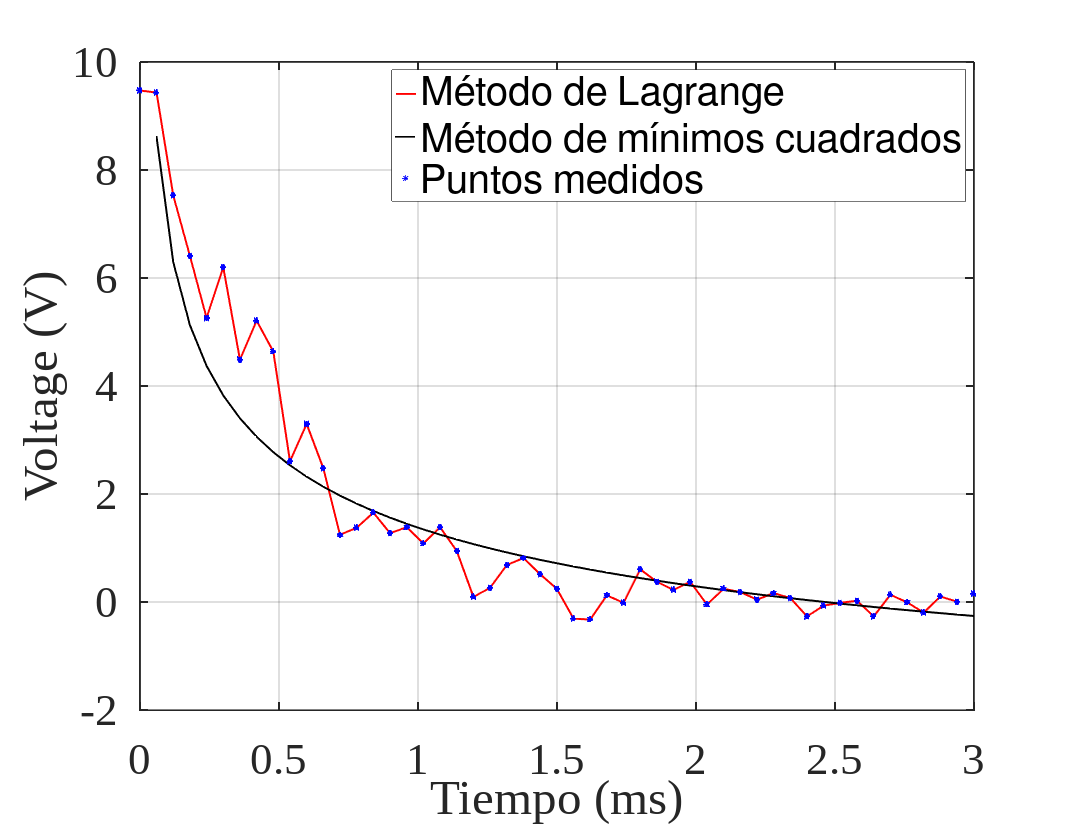
\includegraphics[width=0.43\textwidth]{./plots/ej1-a-plot-0.png}
%\caption{}
\label{fig:fig}
\end{figure}

\begin{figure}[H]
\centering
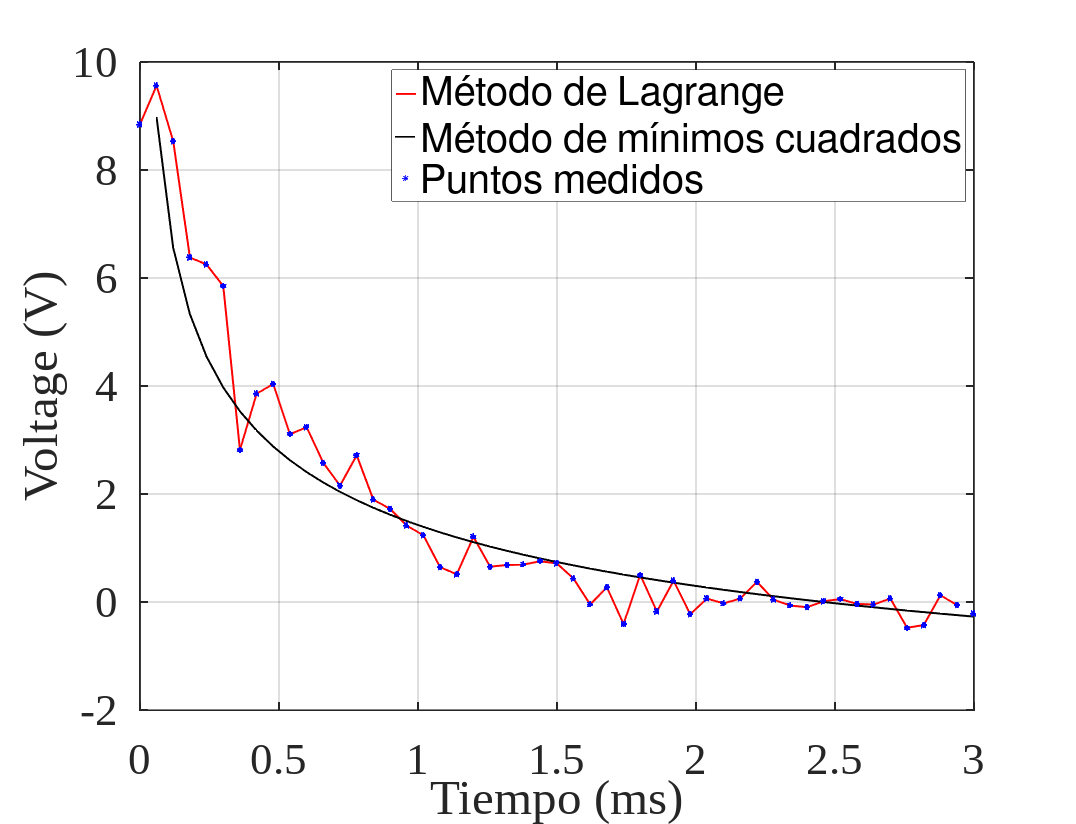
\includegraphics[width=0.43\textwidth]{./plots/ej1-a-plot-1.png}
%\caption{}
\label{fig:fig}
\end{figure}

\begin{figure}[H]
\centering
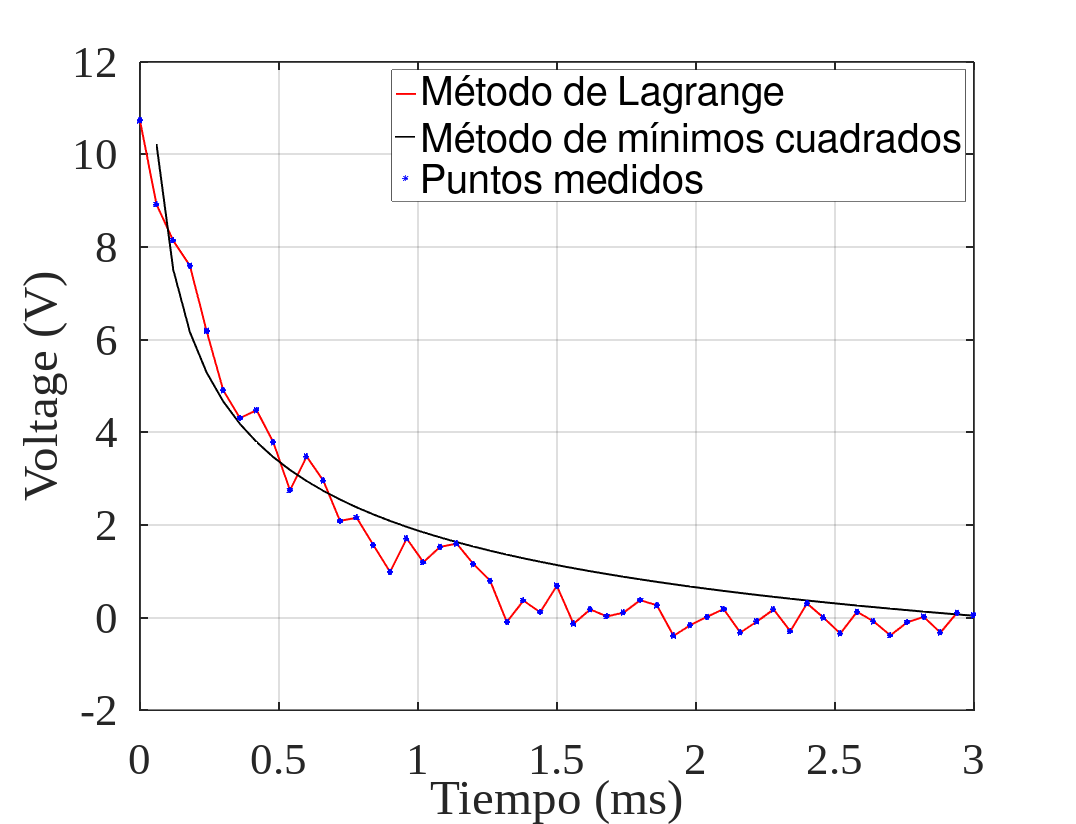
\includegraphics[width=0.43\textwidth]{./plots/ej1-a-plot-2.png}
%\caption{}
\label{fig:fig}
\end{figure}

\section{Ejercicio 2}

\subsection{Marco Te\'orico}

Para aproximar $\bar{R}$ se midi\'o $u_{s}(t)$ y $i_{R}(t)$, y a partir de la ley de ohm:
    \[ V_{R} = \bar{R}I_{R} \] 
    Se puede aplic\'o el m\'etodo de m\'inimos cuadrados y se obtuvo una aproximaci\'on de $\bar{R}$.
    Para poder llegar a un valor consistente se generaron 49 repeticiones de \'este m\'etodo y luego se promediaron estos valores, de esta forma se tiene un valor medio de la aproximac\'ion del verdadero valor de la resistencia, est\'o se hizo para el Ej b y c, pues en el a al no haber error no hay cambios al repetir el proceso. 

    \subsection{Resultados}

    En la pr\'oxima tabla se incluyen los primeros 5 valores aproximados y posteriormente el promedio obtenido, en los archivos adjuntos (values-b.mat y values-c.mat) se pueden ver todos los valores calculados.

    \begin{table}[h]
    \begin{center}
    \begin{tabular}{|c||c|}
    \hline
    Ej. b & Ej. c \\ 
    \hline
    1.8893689700835241 & 1.8893689700835241 \\ 
    \hline
    1.9458937425267899 & 1.9458937425267899 \\ 
    \hline
    1.929197846439076 & 1.929197846439076 \\ 
    \hline
    1.8054188637685247 & 1.8054188637685247 \\ 
    \hline
    2.0941426320507293 & 2.0941426320507293 \\ 
    \hline
    \end{tabular}
    \end{center}
    \caption{Valores de $\bar{R}$ aproximados}
    \label{tab:simple}
    \end{table}

    \begin{table}[h]
    \begin{center}
    \begin{tabular}{|c||c||c|}
    \hline
    Ej. a & Ej. b & Ej. c \\ 
    \hline
    2.0036 & 1.889880012621626 & 2.0011405711954762 \\
    \hline
    \end{tabular}
    \end{center}
    \caption{Promedios obtenidos de $\bar{R}$}
    \label{tab:simple}
    \end{table}

    Como se puede observar en el Ej. c al tomar un intervalo m\'as pequño se tiene una mejor aproximaci\'on al valor verdadero teniendo los errores relativos porcentuales:

    \begin{table}[h]
    \begin{center}
    \begin{tabular}{|c||c||c||c|}
    \hline
    & Ej. a & Ej. b & Ej. c \\ 
    \hline
        Error & 0.1800\% & 5.5060\% & 0.057029\% \\
    \hline
    \end{tabular}
    \end{center}
    \caption{Errores relativos porcentuales de $\bar{R}$}
    \label{tab:simple}
    \end{table}

\section{Ejercicio 3}

\subsection{Marco Te\'orico}
Para aproximar los valores de L y C si hizo medio del m\'etodo de Simpson 3/8, para integrar:
\[ \int_{t_{0}}^{t} i_{c}(\tau) \,d\tau \]
y
\[ \int_{t_{0}}^{t} u_{L}(\tau) \,d\tau \]
Pues a partir de ecuaciones f\'isicas conocidas se tienen las relaciones:
\[ C = \frac{\int_{t_{0}}^{t} u_{L}(\tau) \,d\tau}{u_{c}(t)} = c(t) \]
\[ L = \frac{\int_{t_{0}}^{t} u_{L}(\tau)}{i_{L}(t)} \,d\tau = l(t) \]
tambi\'en:
\[ i_{C} = i_{L} + i_{R} \]
\[ u_{L} = u_{S} = u_{R} \]
\[ u_{C} = u_{e} - u_{s} \]
Por lo tanto s\'olo integrando y despejando de las ecuaciones se pueden aproximar ambas magnitudes.
Se eligi\'o el m\'etodo de Simpson 3/8 pues tiene una precisi\'on suficiente para el caso y es facilmente implementable.

\subsection{Resultados}

Todos los datos que se resumen en la siguiente table se pueden encontrar en los archivos adjuntos.

    \begin{table}[h]
    \begin{center}
    \begin{tabular}{|c||c||c|}
    \hline
    & L &  C \\ 
    \hline
        Promedio & 0.093531236156927489 & 0.00023562271769011871 \\
    \hline
    Error & 6.46\% & 5.75\% \\
    \hline
    \end{tabular}
    \end{center}
    \caption{Errores relativos porcentuales}
    \label{tab:simple}
    \end{table}
    
\section{Ejercicio 4}

\subsection{Marco Te\'orico}

Para poder resolver la ecuaci\'on diferencial ordinaria de orden dos que se presenta como soluci\'on a la tensi\'on de salida $u_{S}(t)$ del circuito se plante\'o un sistema de dos ecuaciones (1 y 2) que reducen en un orden la misma, de \'esta forma se pudieron aplicar los m\'etodos de soluci\'on de EDO\footnote{Ecuaci\'on diferencial ordinaria} de Euler, Taylor, Adams Bashforth y Runge Kutta.
\[ \frac{ \partial^2 {u_{S}(t)}}{\partial t^2} + \frac{1}{RC}\frac{\partial{u_{S}(t)}}{\partial{t}} + \frac{u_{S}(t)}{LC} = \frac{\partial^2{u_{e}(t)}}{{\partial{t^2}}} \]
con las condiciones iniciales:
\[ \begin{cases} u_{S}(t_{0}) = 0 \\ u'_{S}(t_{0}) = A2\pi$f$ \end{cases} \] 
Resulta en \ldots
\[ \begin{cases} y_0 = u_{S}(t) \\ y_1 = u'_{S}(t) = y'_0 \\ y_2 = u''_{S}(t) = y'_1 = y''_0 \\ y'_1 = y_2 (1) \\ y'_2 = - \frac{1}{RC} y_2 - \frac{1}{LC} y_1 (2) \\ u_{S}(t_{0}) = 0 \\ u'_{S}(t_{0}) = A2\pi$f$ \end{cases} \]
La forma en que se resulven estas dos nuevas EDOs es pasando como primer valor para $y_0$ e $y_1$ las condiciones iniciales, $u_{S}(t_{0})$ y $u'_{S}(t_{0})$ respectivamente, y luego se deben resolver en simult\'aneo, aplicando el m\'etodo que se quiera; pues al ser un sistema de ecuaciones ambas se relacionan, y de otra forma no se podr\'ian resolver.

\subsection{Resultados}

Como se pueden observar en los siguientes gr\'aficos los m\'etodos convergen de forma muy similar a exepc\'ion de Adams Bashforth que tiene un clara divergencia.

\begin{figure}[H]
\centering
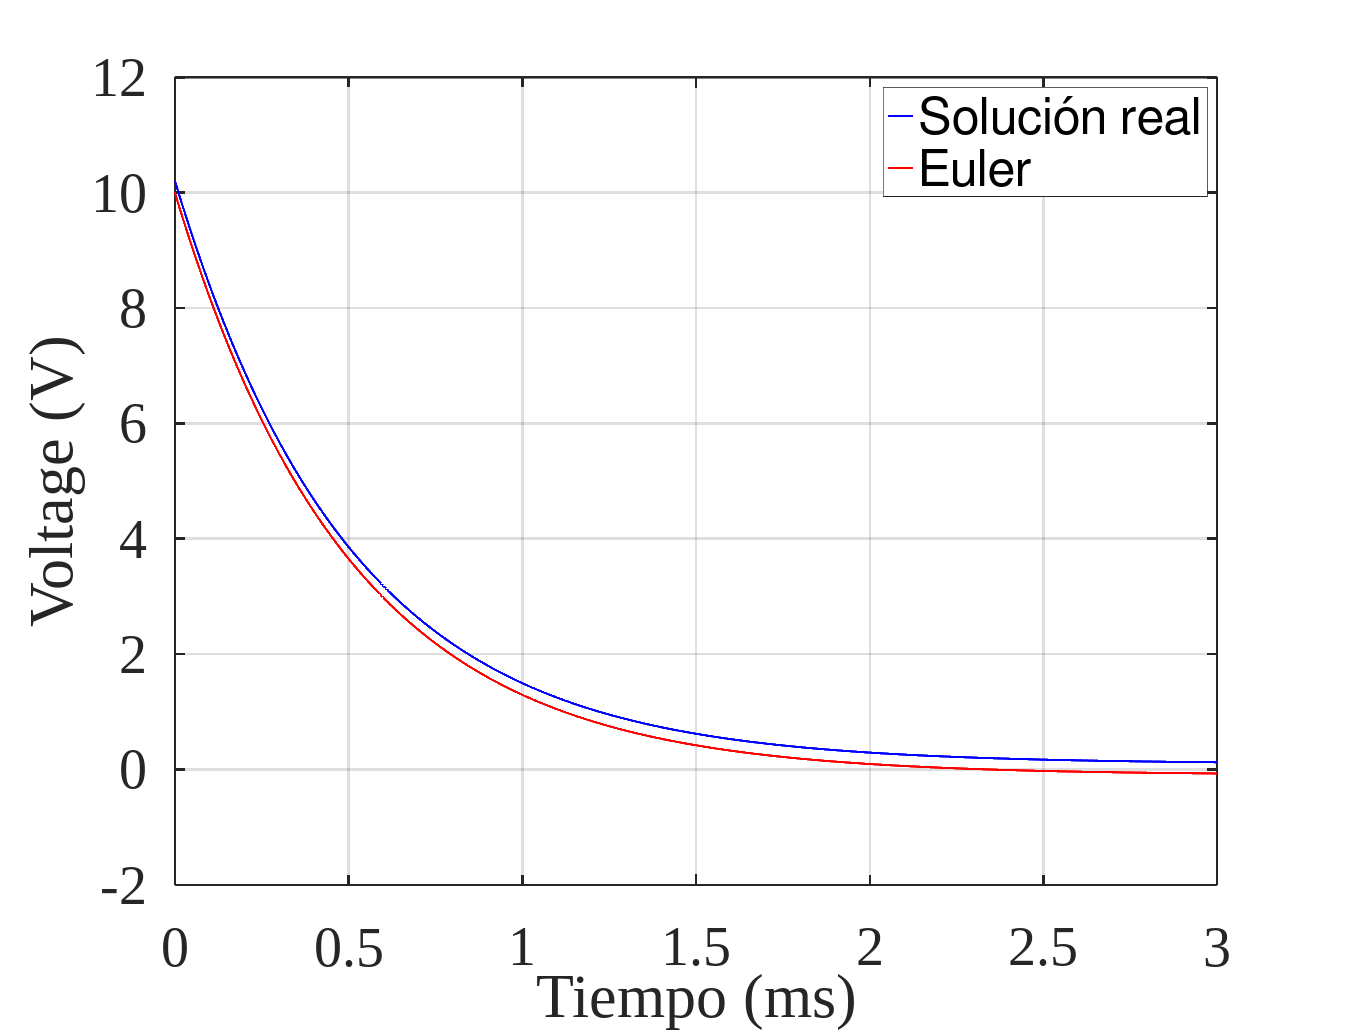
\includegraphics[width=0.43\textwidth]{../plots/ej4/ej4-metodos-3.png}
\end{figure}

\begin{figure}[H]
\centering
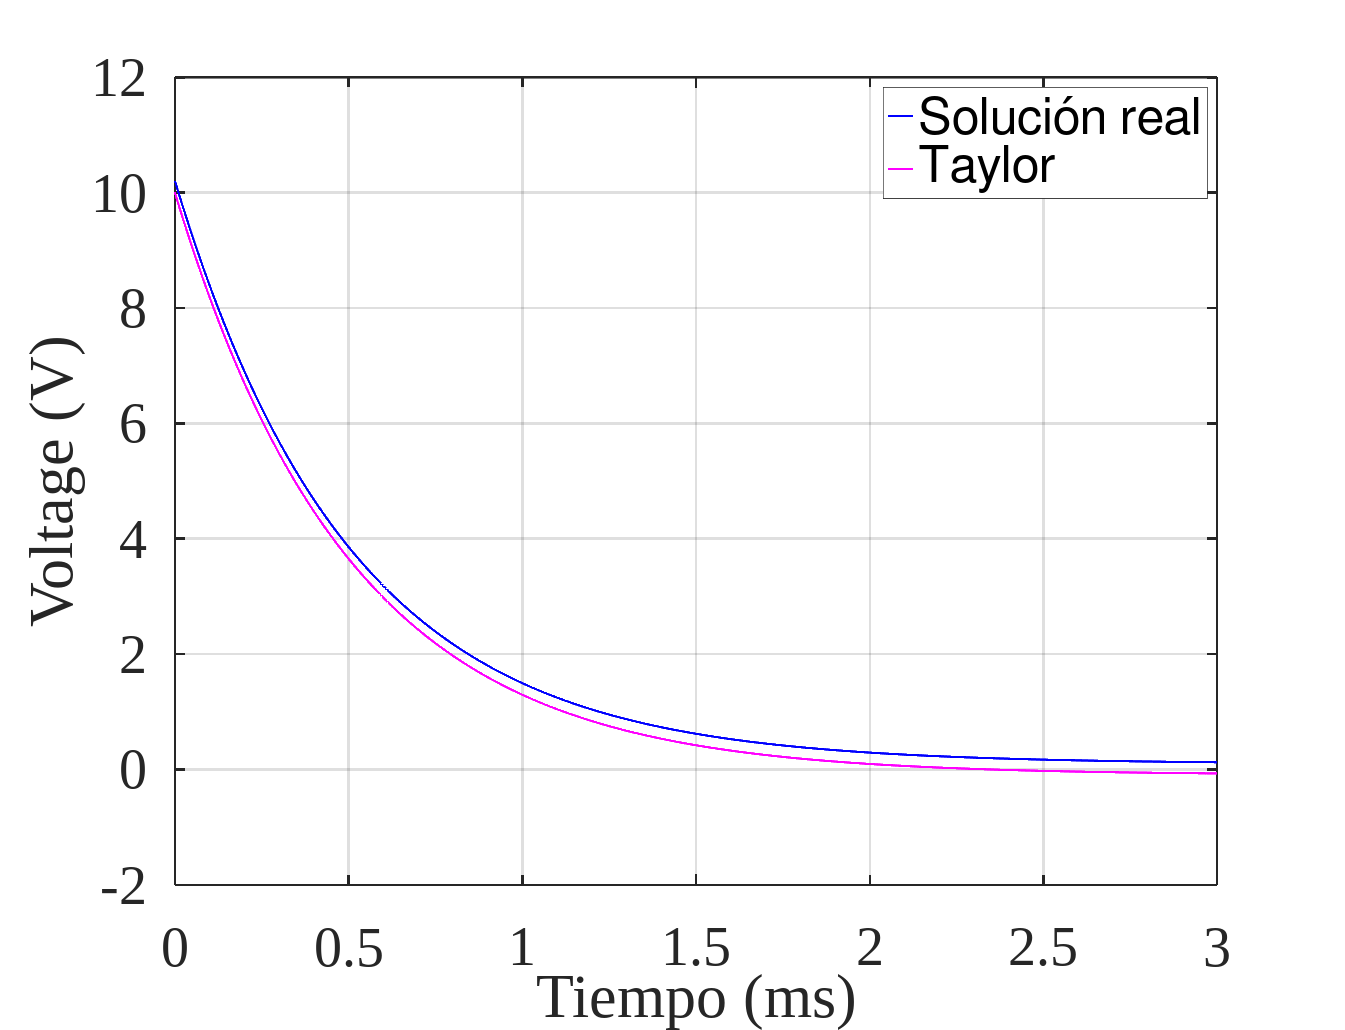
\includegraphics[width=0.43\textwidth]{../plots/ej4/ej4-metodos-4.png}
\end{figure}

\begin{figure}[H]
\centering
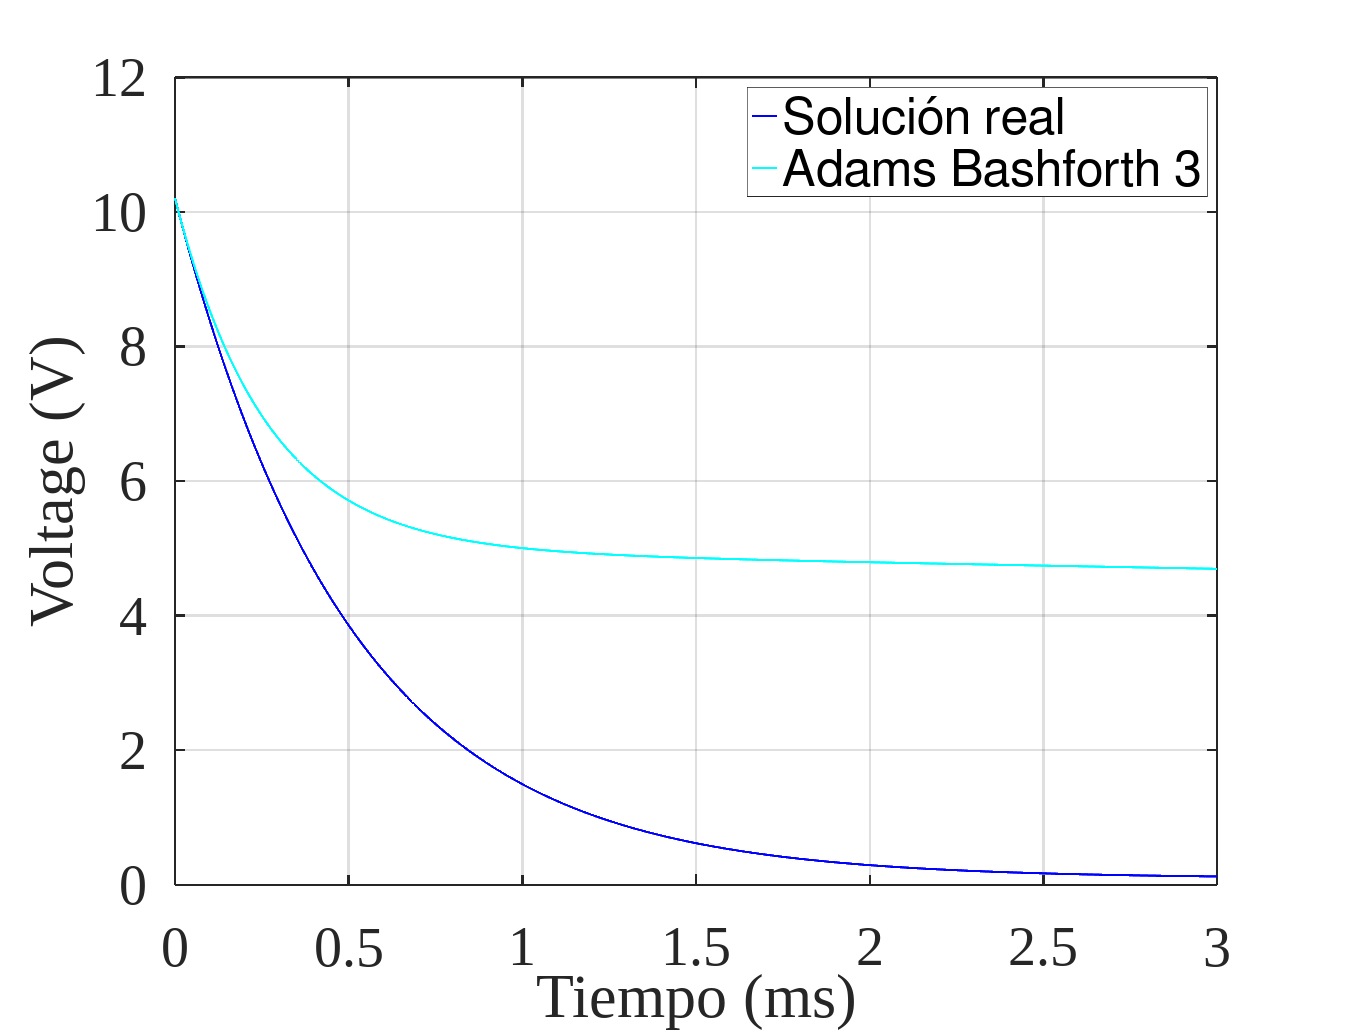
\includegraphics[width=0.43\textwidth]{../plots/ej4/ej4-metodos-5.png}
\end{figure}

\begin{figure}[H]
\centering
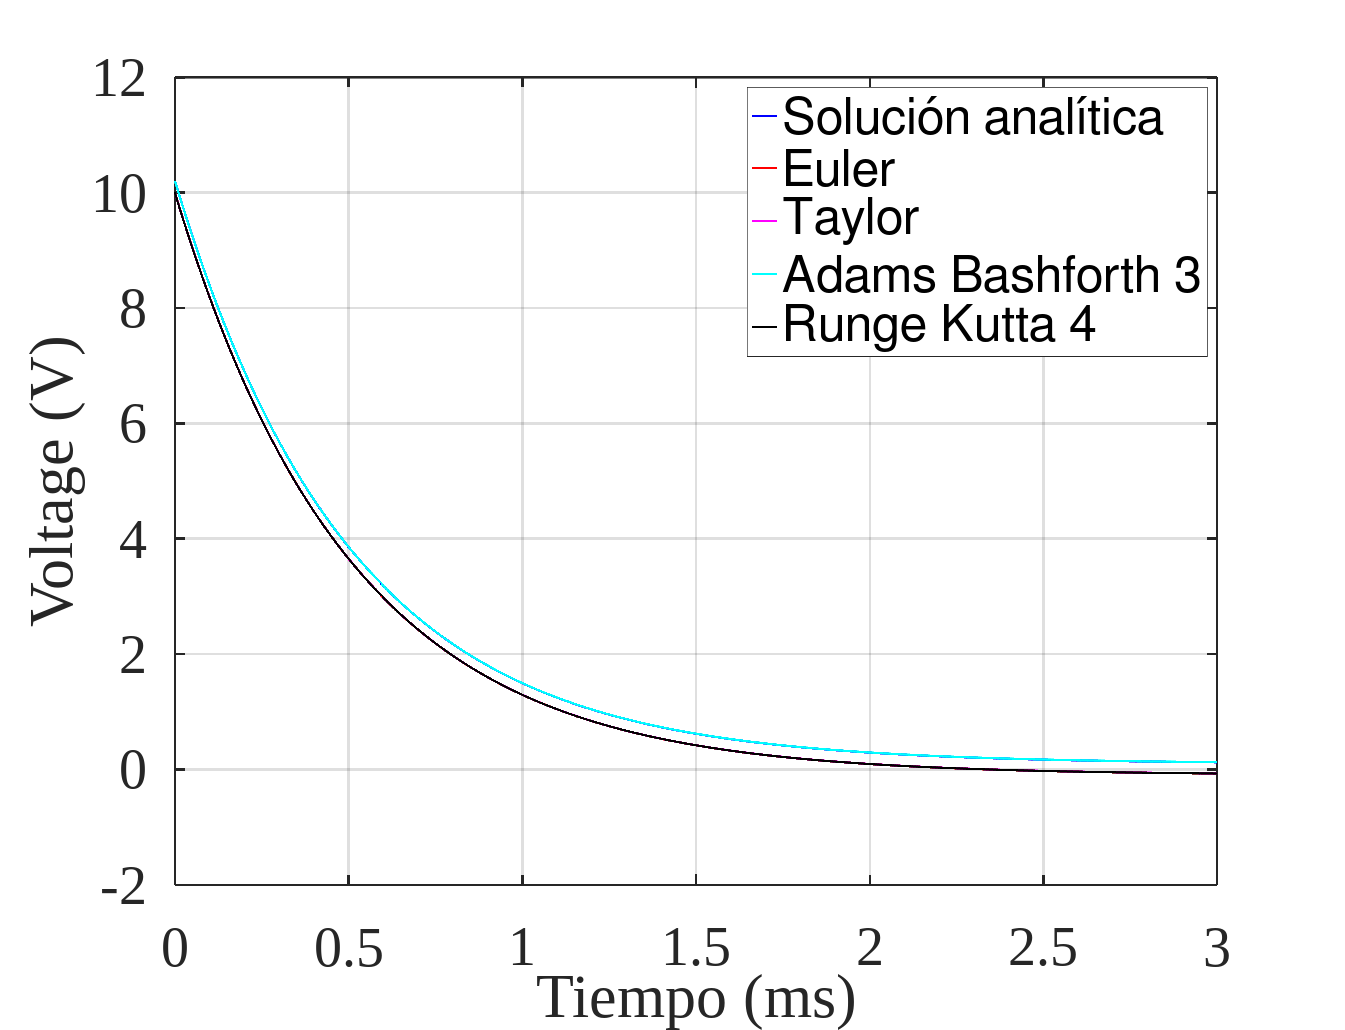
\includegraphics[width=0.43\textwidth]{../plots/ej4/ej4-metodos-2.png}
\end{figure}

\begin{figure}[H]
\centering
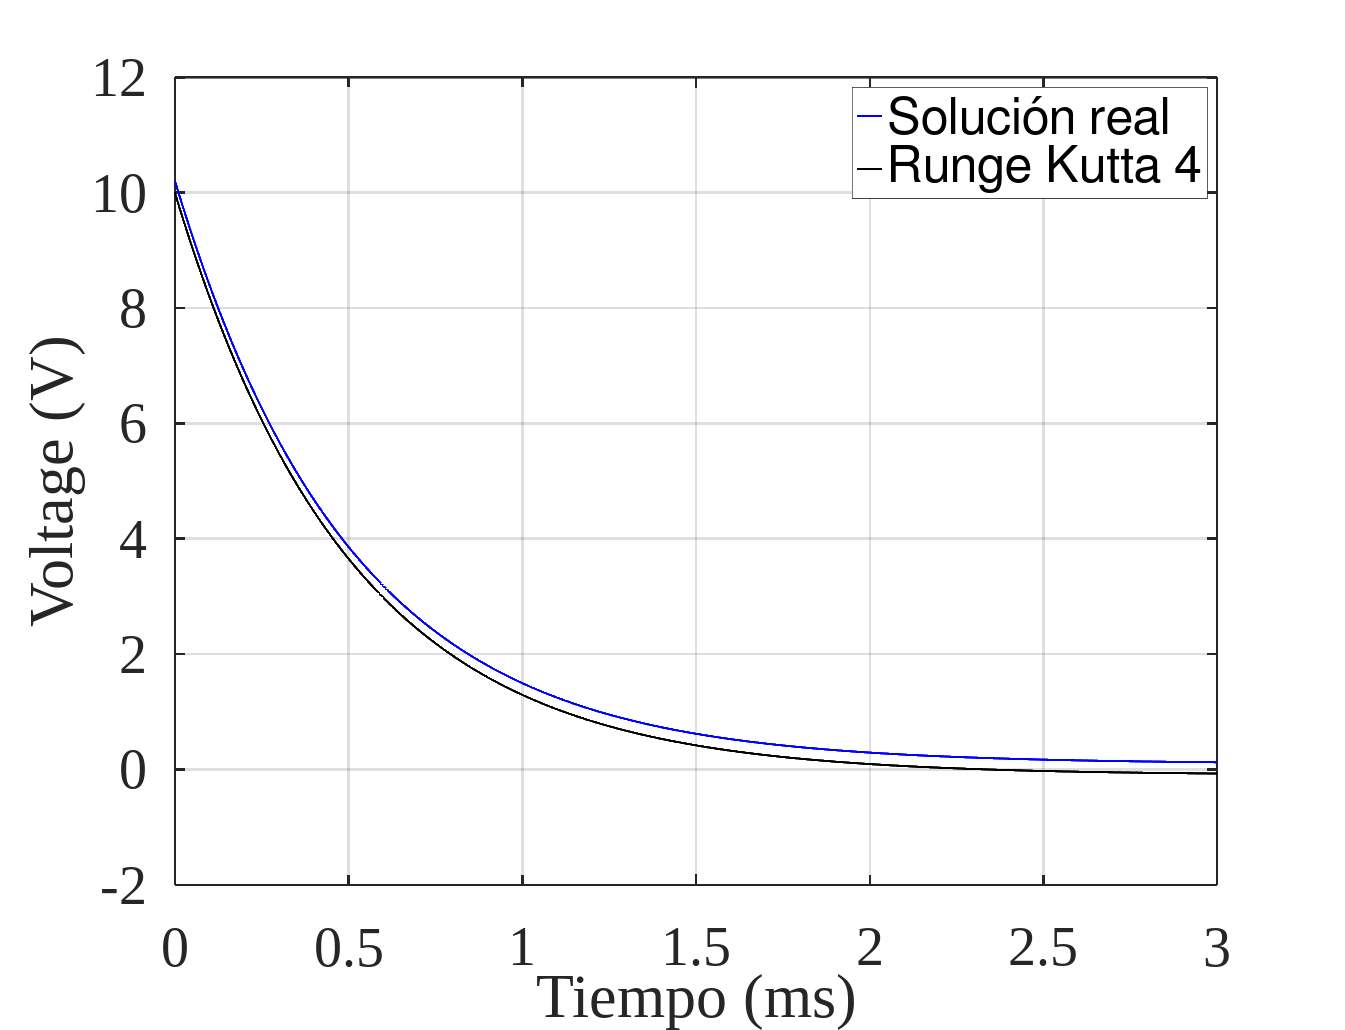
\includegraphics[width=0.43\textwidth]{../plots/ej4/ej4-metodos-6.png}
\end{figure}

\begin{figure}[H]
\centering
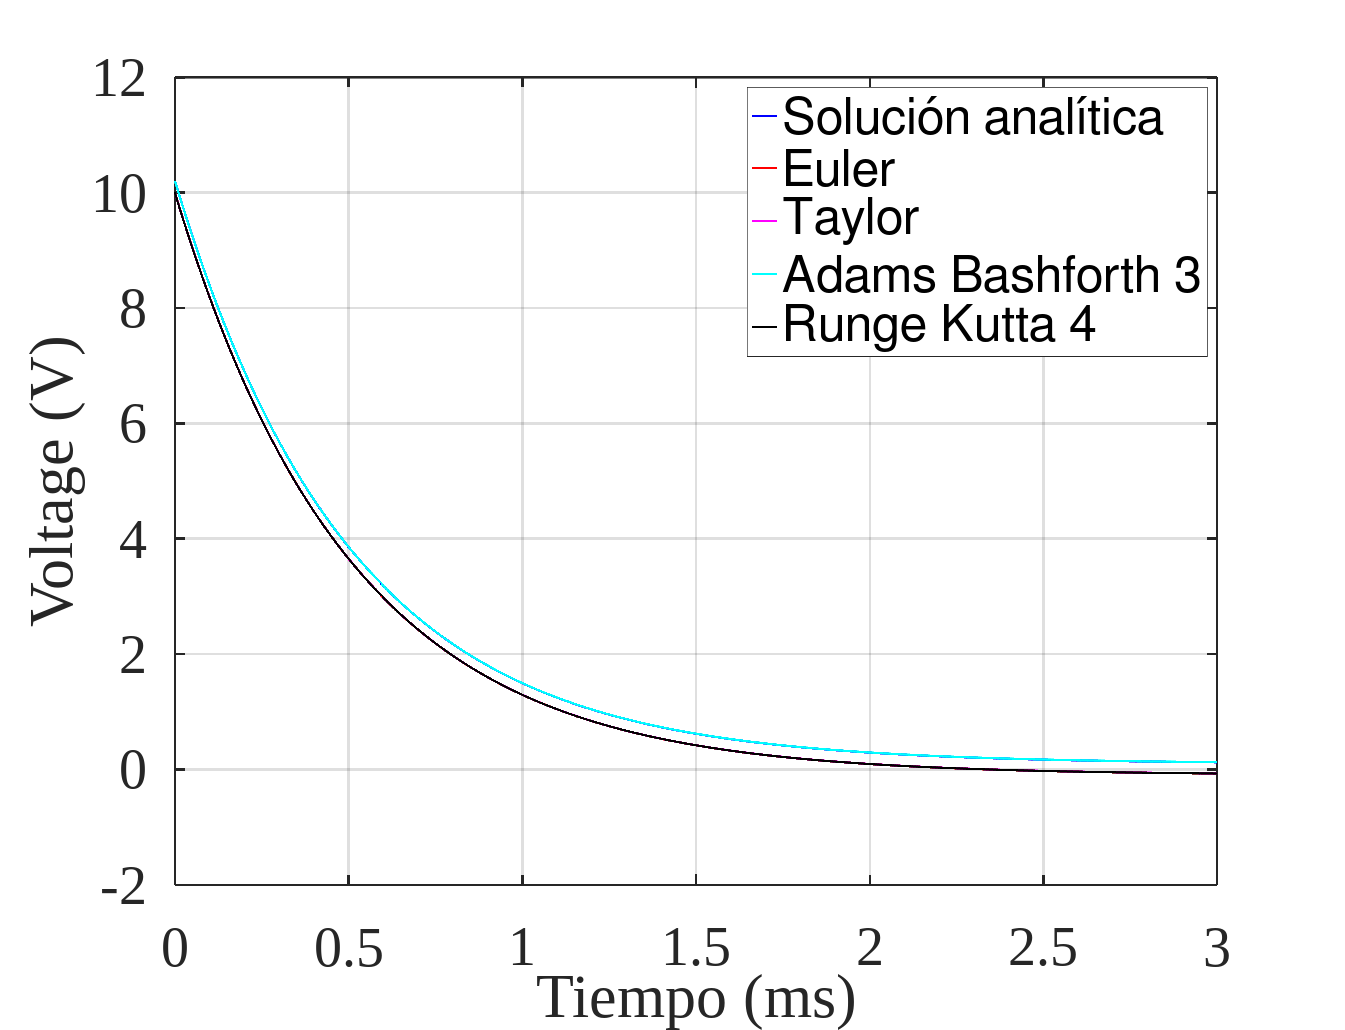
\includegraphics[width=0.43\textwidth]{../plots/ej4/ej4-metodos-2.png}
\end{figure}

\begin{text}Con los errores relativos porcentuales\ldots \end{text}

\begin{figure}[H]
\centering
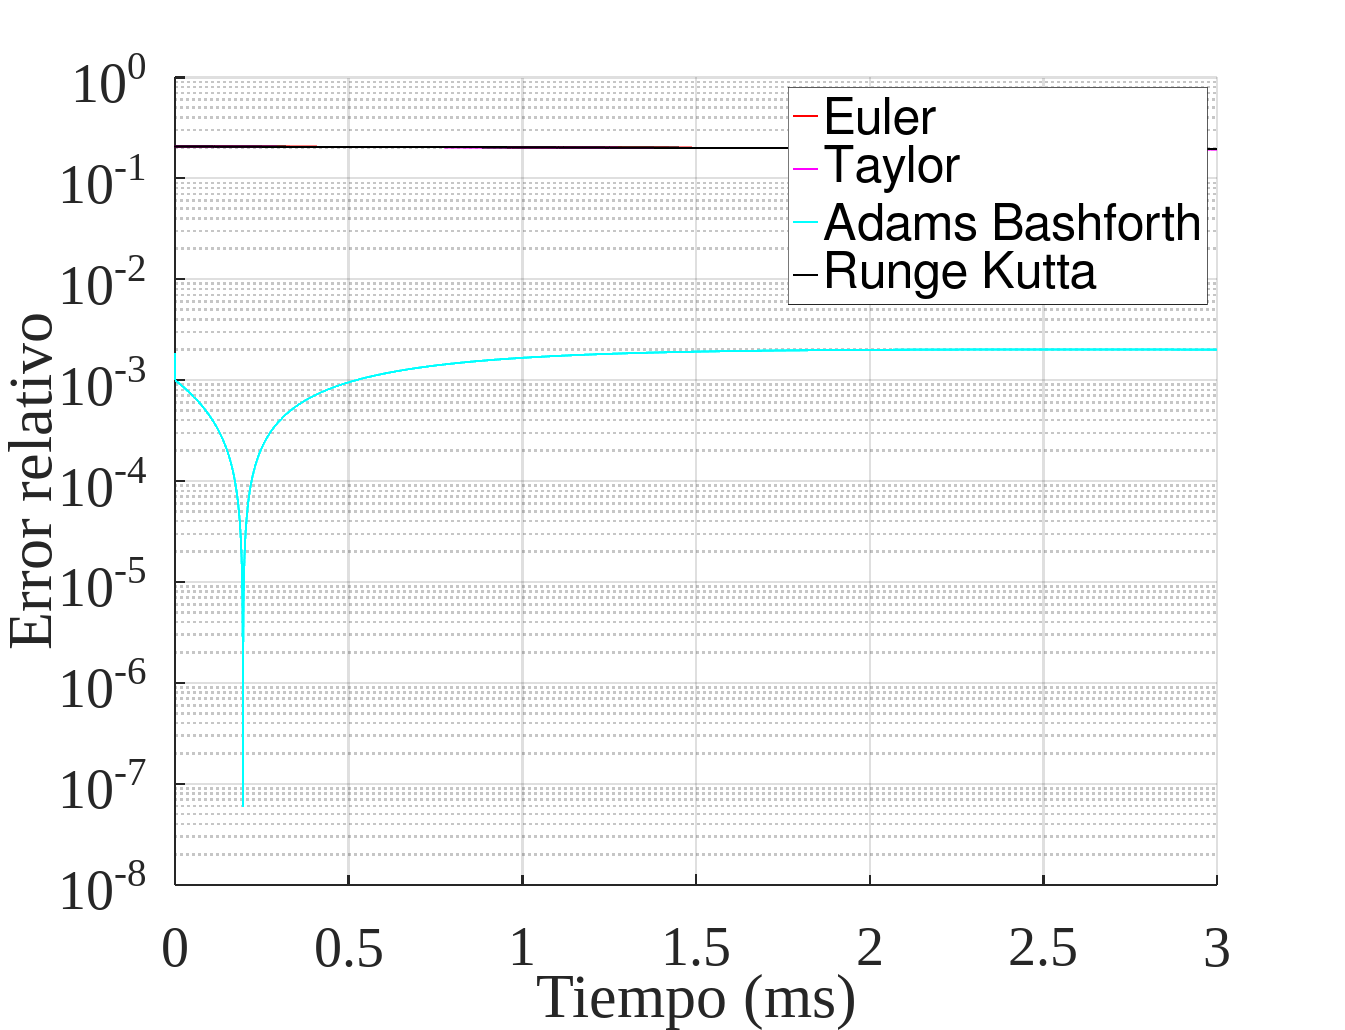
\includegraphics[width=0.43\textwidth]{../plots/ej4/ej4-errores-1.png}
\label{fig:fig}
\end{figure}

\begin{figure}[H]
\centering
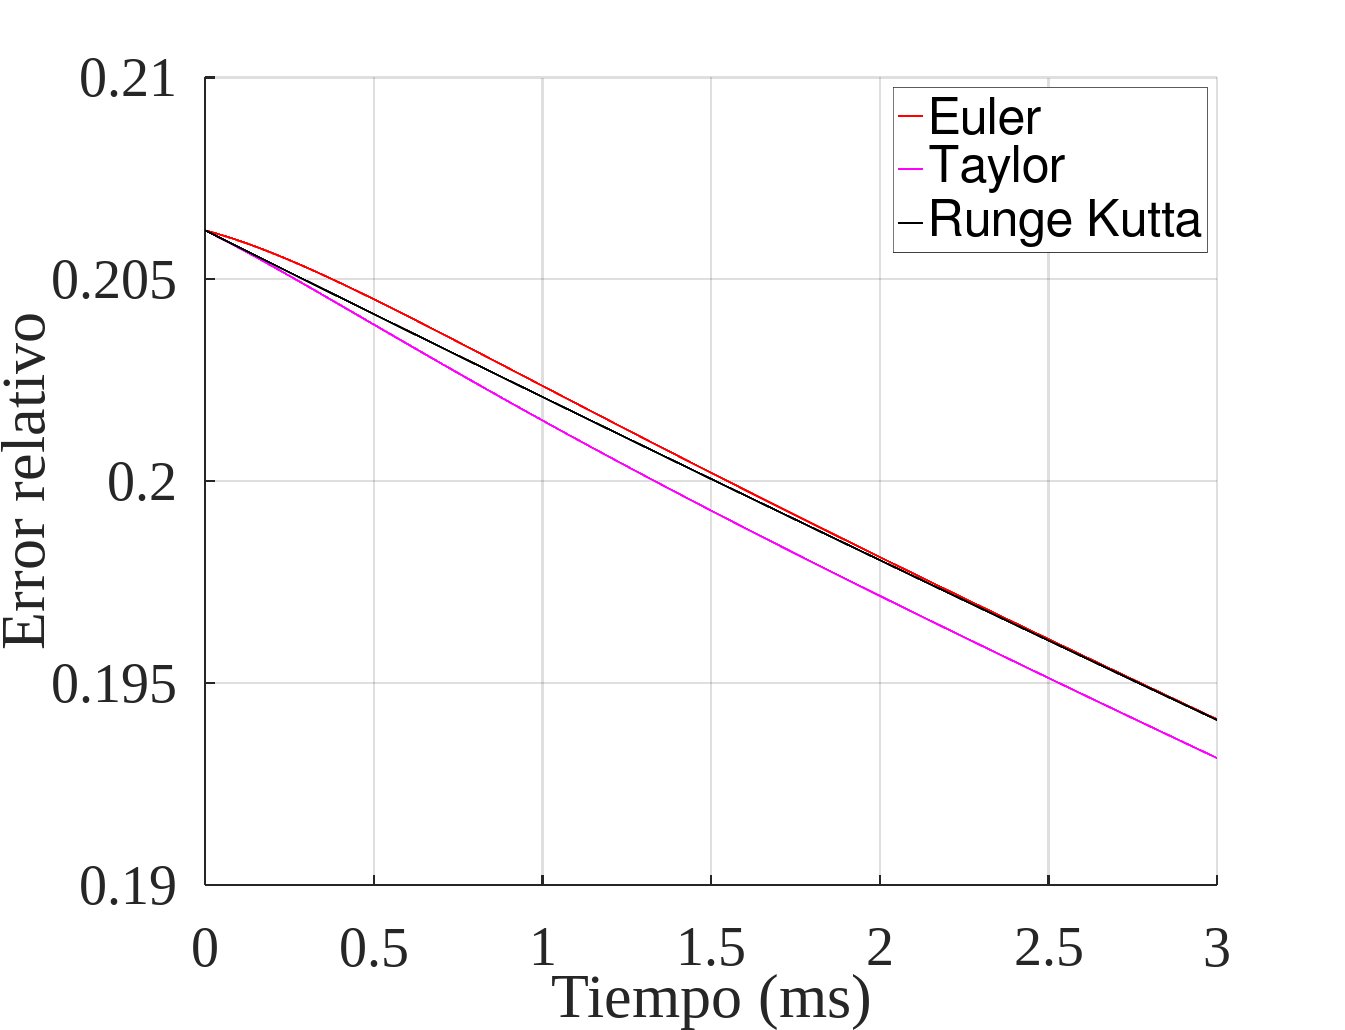
\includegraphics[width=0.43\textwidth]{../plots/ej4/ej4-errores-2.png}
\label{fig:fig}
\end{figure}

En conclusi\'on el mejor m\'etodo para las condiciones presentes es el de Taylor de orden 2, pues converge con menos error.

\section{Ejercicio 5}

\subsection{Marco Te\'orico}

Basandonos en el mismo marco te\'orico que en el Ejercicio 4 se resuelve la EDO (que ahora es no homog\'enea) con el sistema de EDOs, por lo cual la soluci\'on anal\'itica es diferente, aunque la solucio\'on num\'erica se obtenga con los mismos algoritmos desarrollados en octave previamente (solo se hacen modificaciones para poder calcular m\'as facilmente el resultado ante la variaci\'on de frecuencias).

\subsection{Resultados}

En los siguientes gr\'aficos se muestran c\'omo los m\'etodos aproximan la soluci\'on anal\'itica para 20hz, 200hz, 2000hz y 20000hz. Con \'esto se espera observar el comportamiento de los m\'etodos ante estas variaciones de frecuencia.

\begin{figure}[H]
\centering
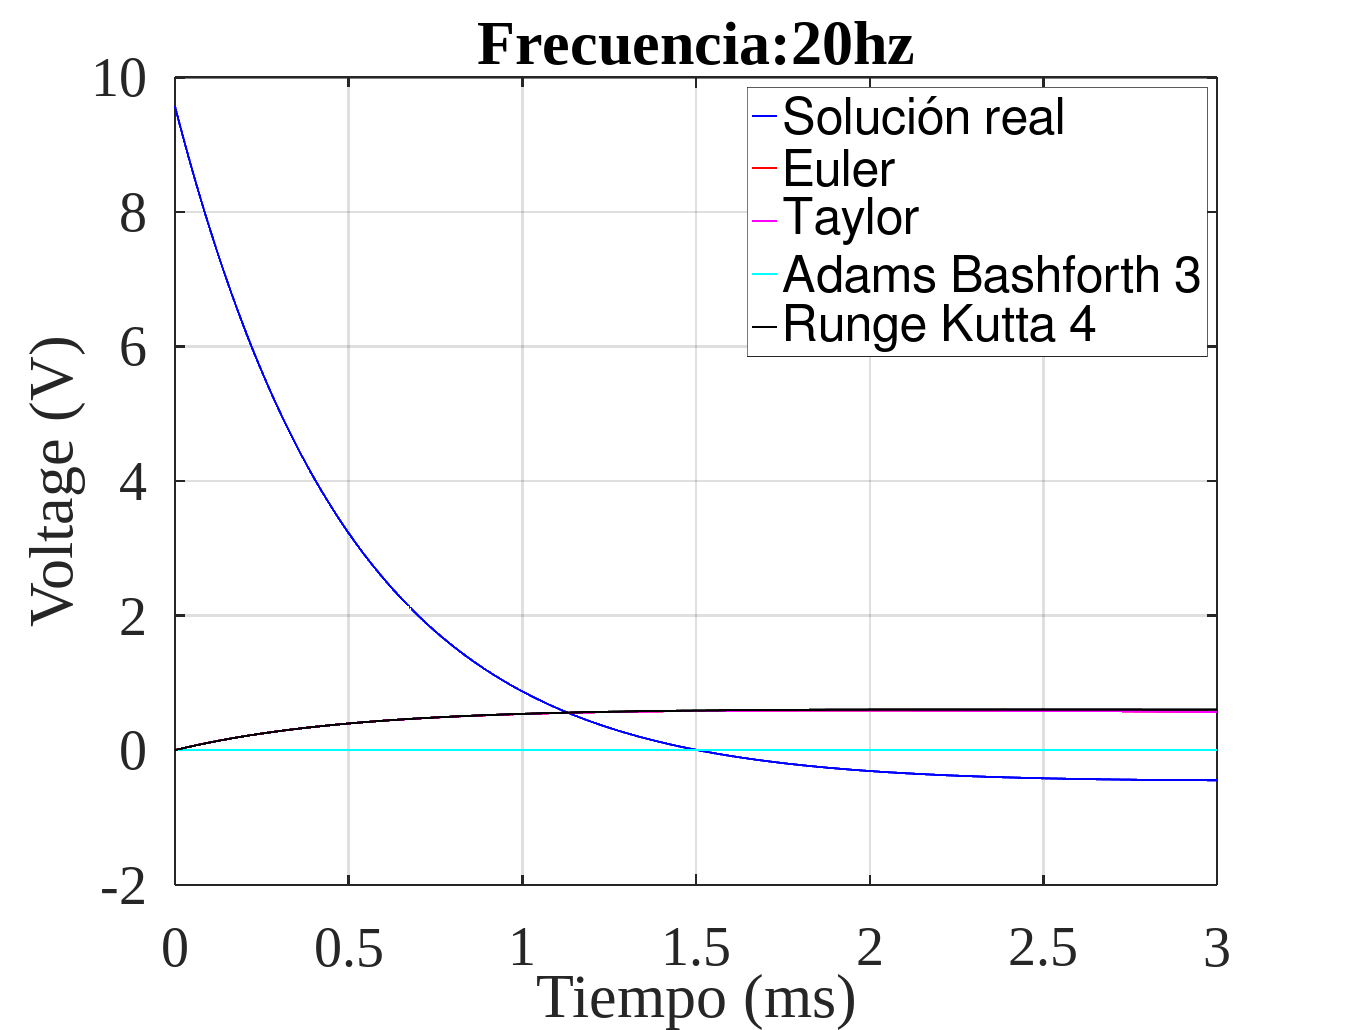
\includegraphics[width=0.43\textwidth]{../plots/ej5/Frecuencia:20hz.png}
\label{fig:fig}
\end{figure}

\begin{figure}[H]
\centering
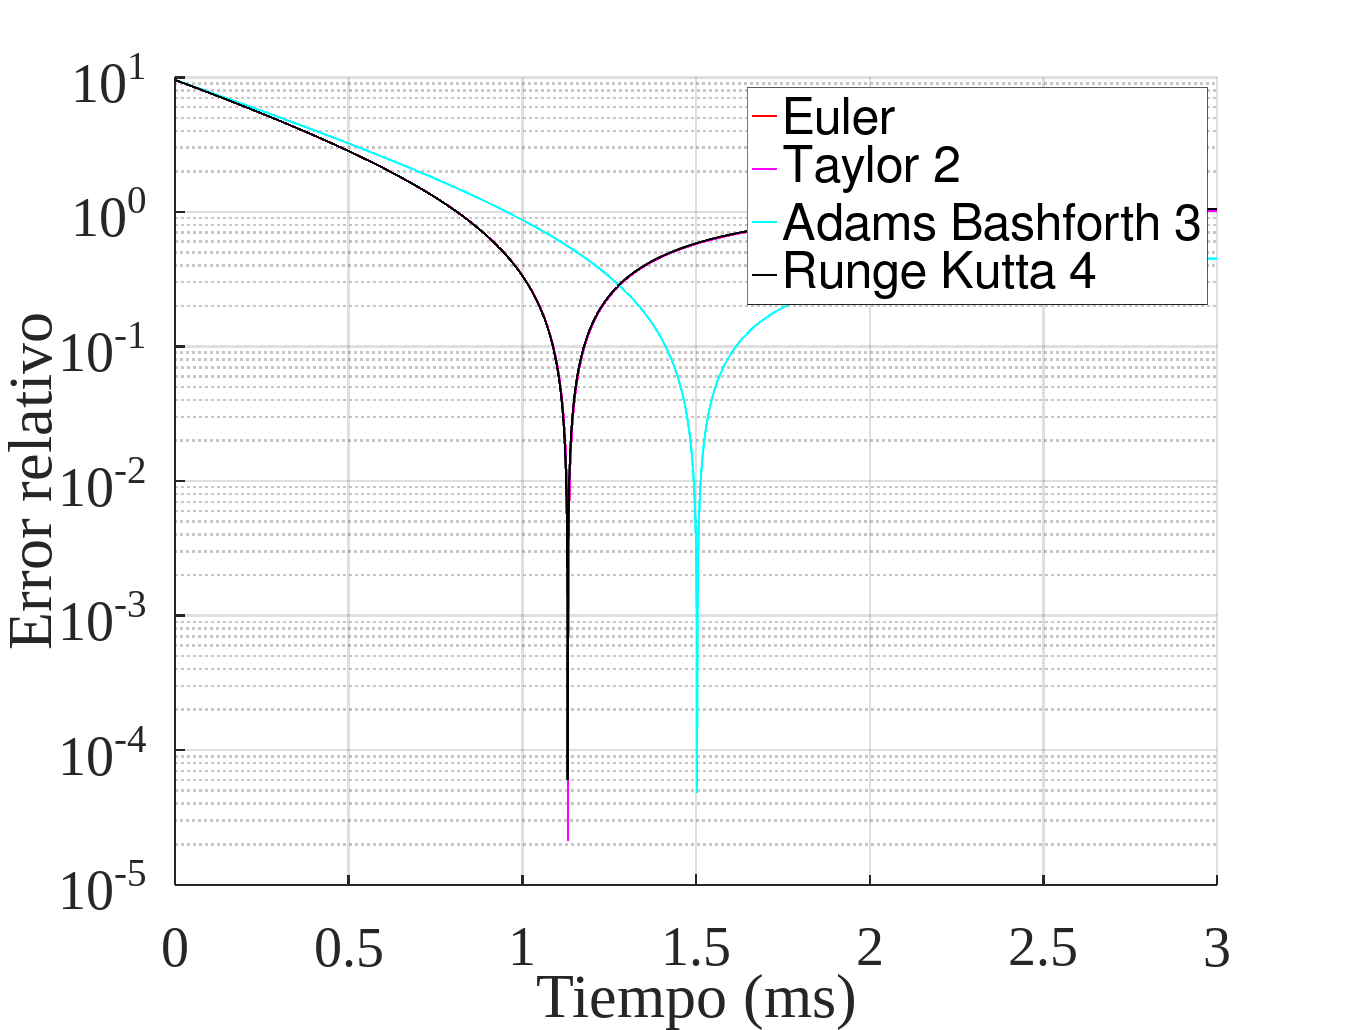
\includegraphics[width=0.43\textwidth]{../plots/ej5/error-20hz.png}
\label{fig:fig}
\end{figure}

\begin{figure}[H]
\centering
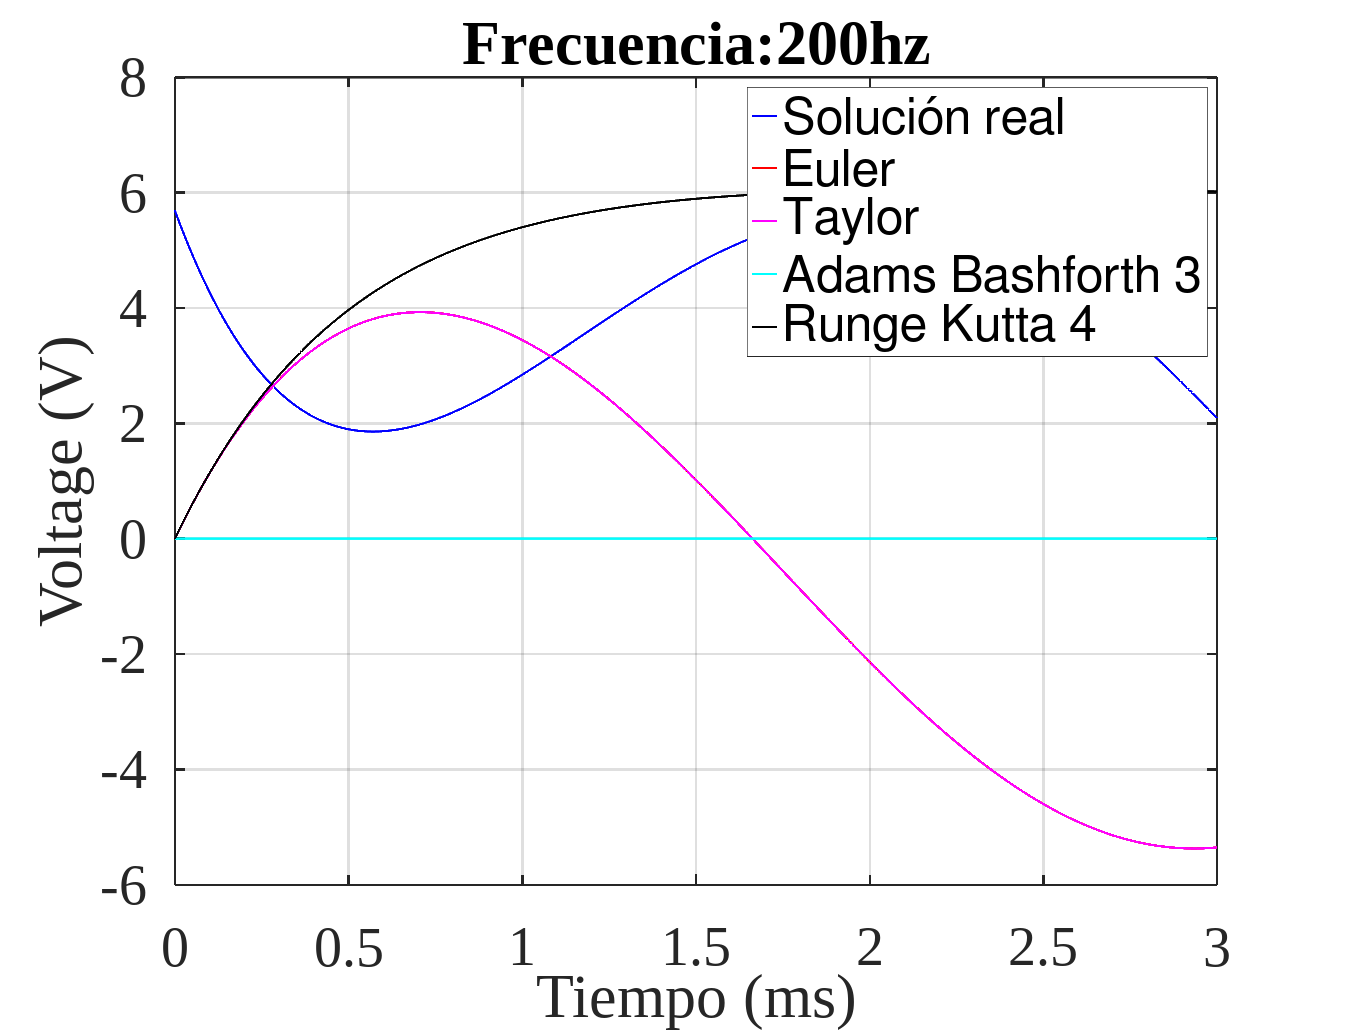
\includegraphics[width=0.43\textwidth]{../plots/ej5/Frecuencia:200hz.png}
\label{fig:fig}
\end{figure}

\begin{figure}[H]
\centering
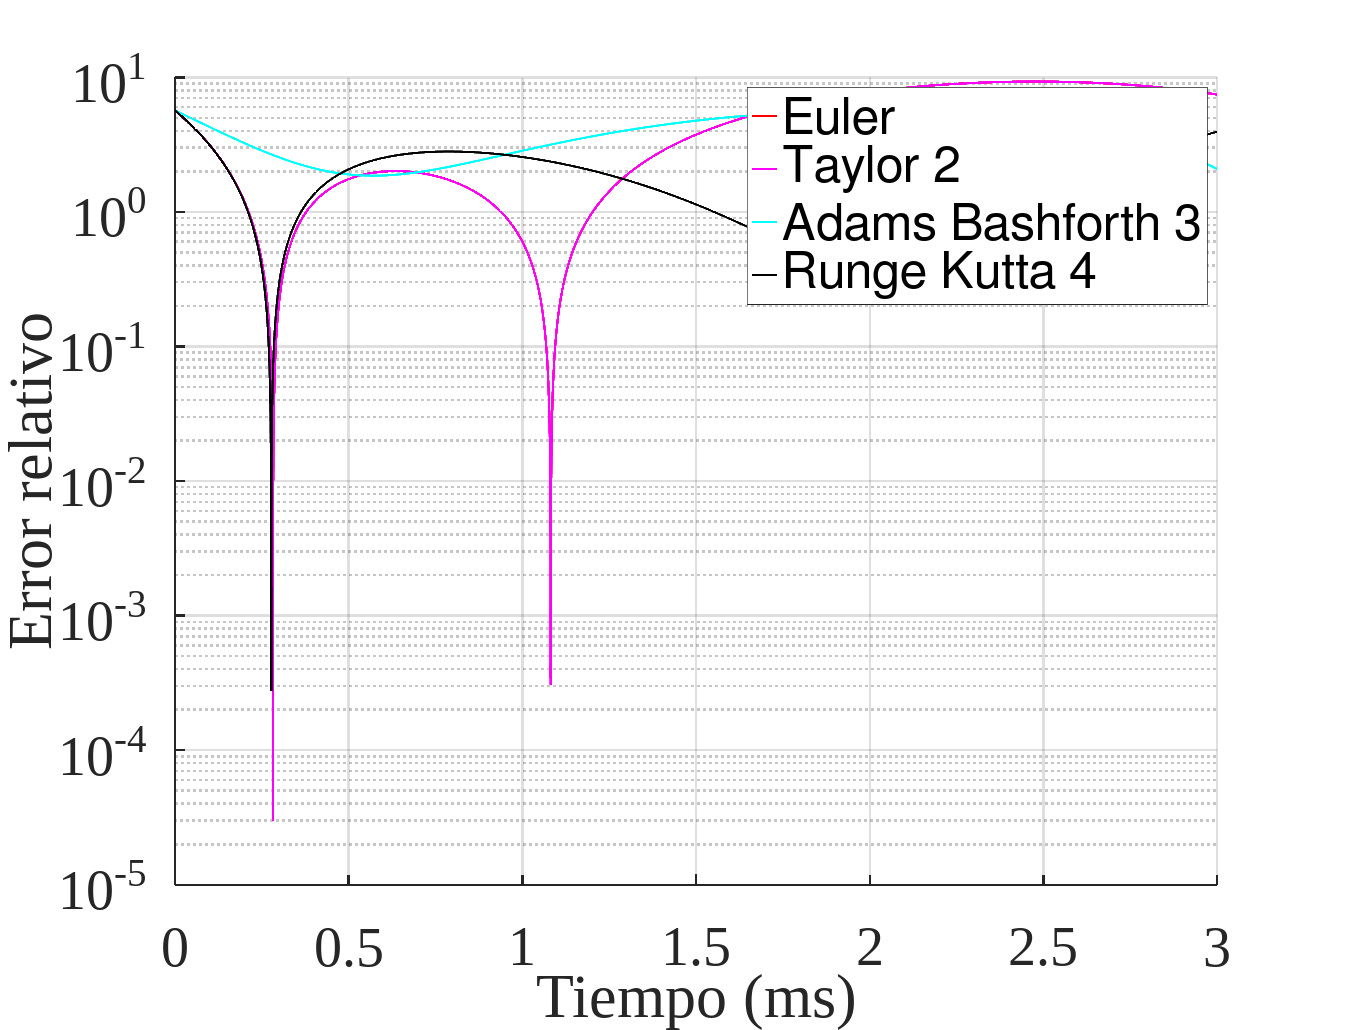
\includegraphics[width=0.43\textwidth]{../plots/ej5/error-200hz.png}
\label{fig:fig}
\end{figure}

\begin{figure}[H]
\centering
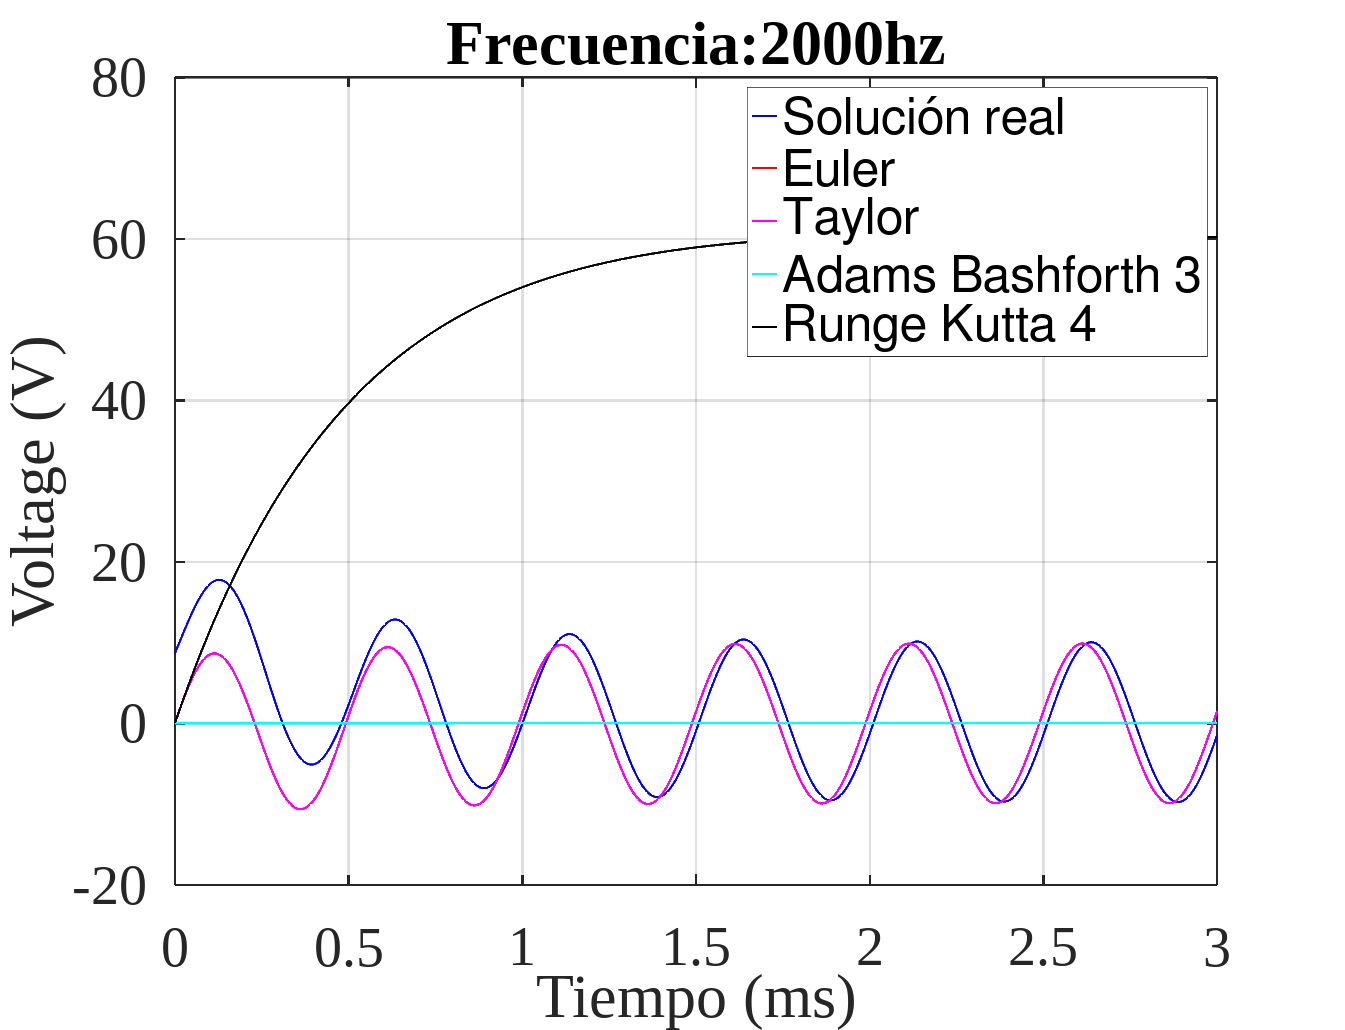
\includegraphics[width=0.43\textwidth]{../plots/ej5/Frecuencia:2000hz.png}
\label{fig:fig}
\end{figure}

\begin{figure}[H]
\centering
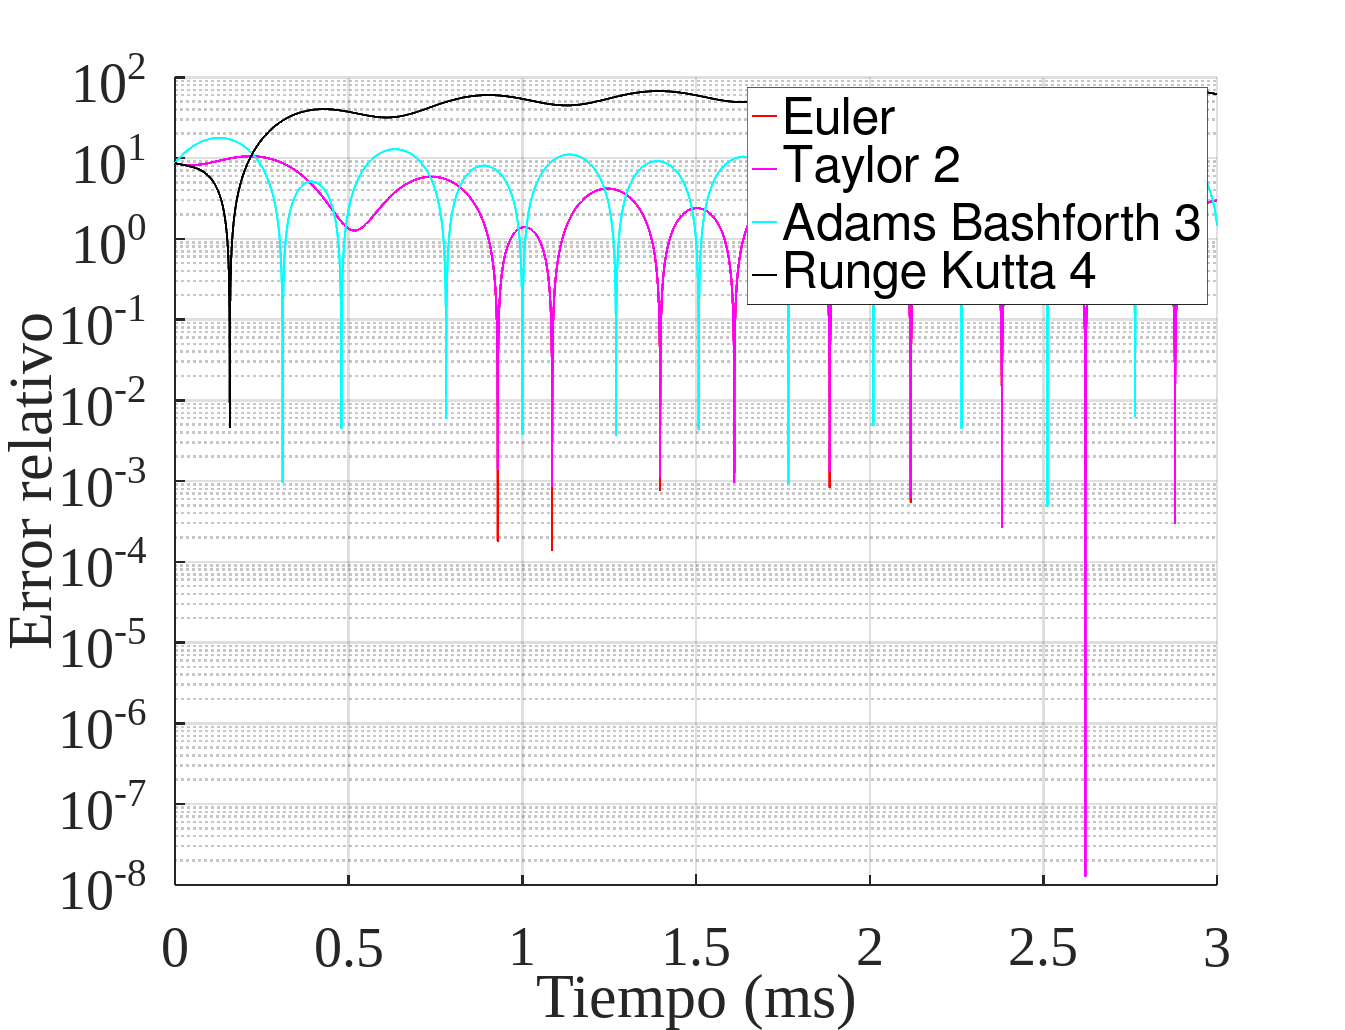
\includegraphics[width=0.43\textwidth]{../plots/ej5/error-2000hz.png}
\label{fig:fig}
\end{figure}

\begin{figure}[H]
\centering
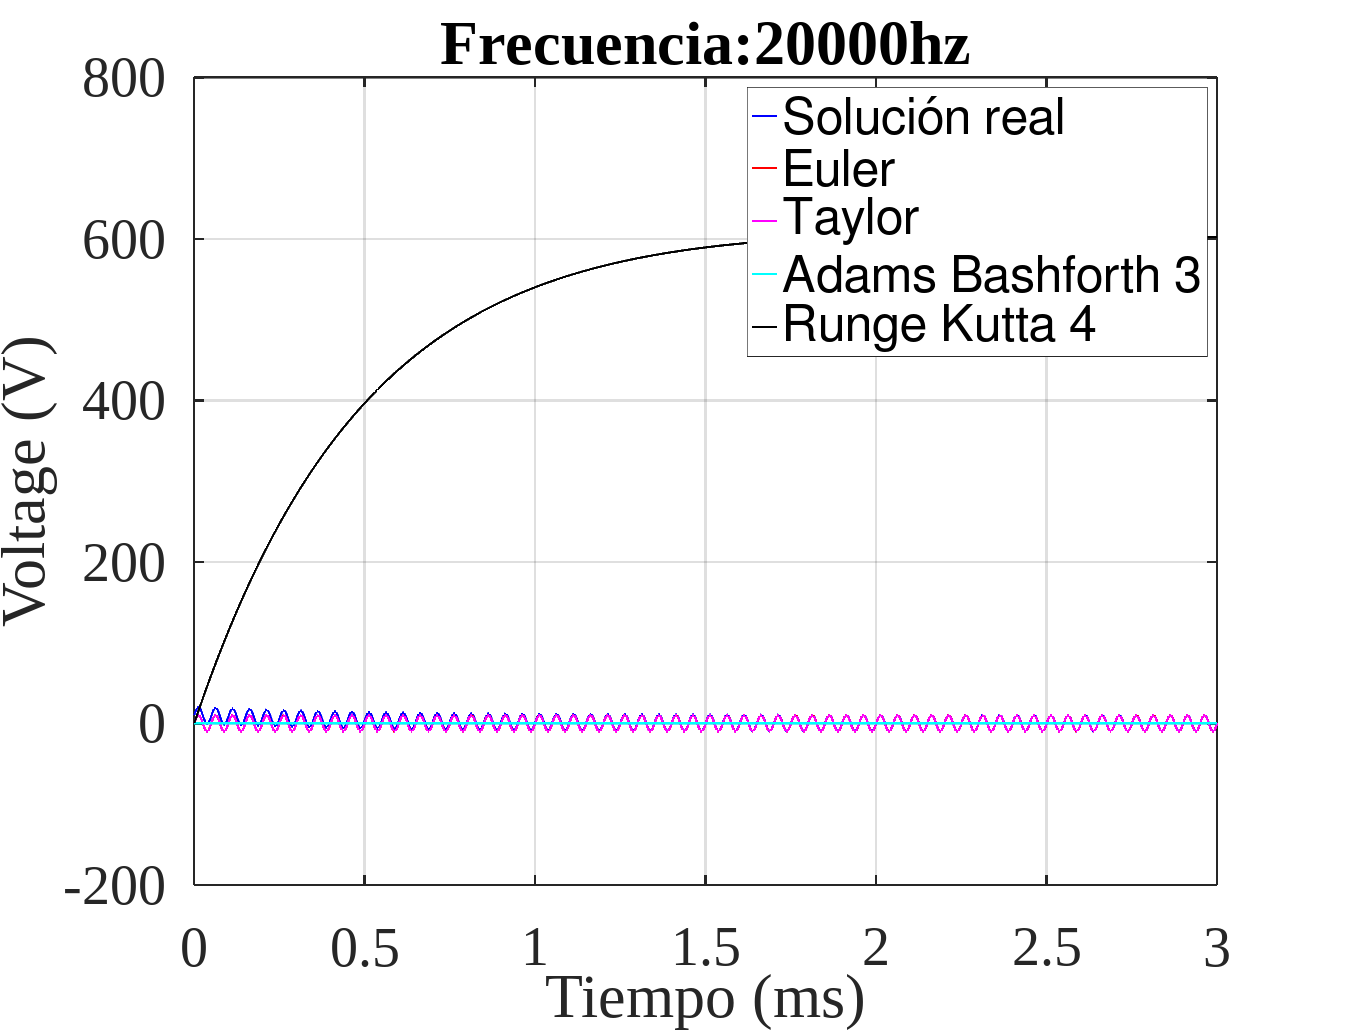
\includegraphics[width=0.43\textwidth]{../plots/ej5/Frecuencia:20000hz.png}
\label{fig:fig}
\end{figure}

\begin{figure}[H]
\centering
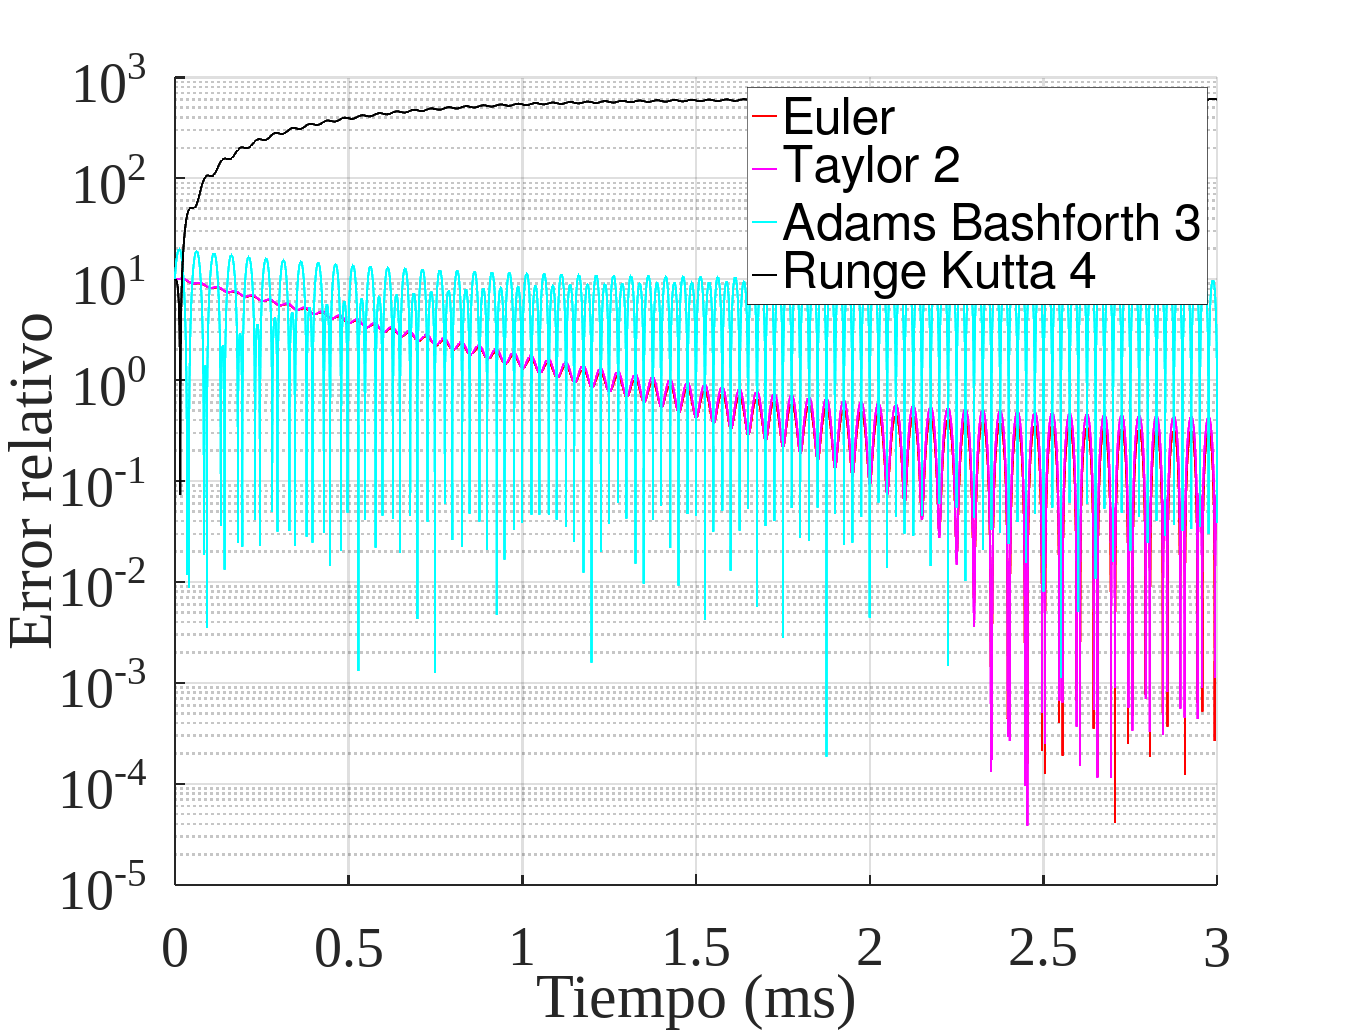
\includegraphics[width=0.43\textwidth]{../plots/ej5/error-20000hz.png}
\label{fig:fig}
\end{figure}

Con estos gr\'aficos podemos ver que el m\'etodo de Runge Kutta 4 termina divergiendo para frecuencias altas, adem\'as Euler y Taylor de orden 2 son superiores a Adams Bashforth para todas las frecuencias estudiadas, y que Taylor sigue siendo el mejor m\'etodo entre estos cuatro, presentando menos error relativo porcentual, aunque, es superior al resto por 'poco' error, por lo que Euler no es para nada una mala alternativa, ya que es m\'as f\'acil de implementar que Taylor de orden 2, porque no requiere el c\'alculo de otra derivada, y tiene menor c\'alculo computacional, por \'estas razones, dependiendo de c\'ual sea el objetivo, Euler puede llegar a ser muy buena soluci\'on.
Ahora para estudiar el comportamiento del circuito ante la variaci\'on de frecuencias se muestran en los siguientes gr\'aficos la comparativa de la señal de entrada $u_{e}(t)$ con respecto de la señal de salida.

\begin{figure}[H]
\centering
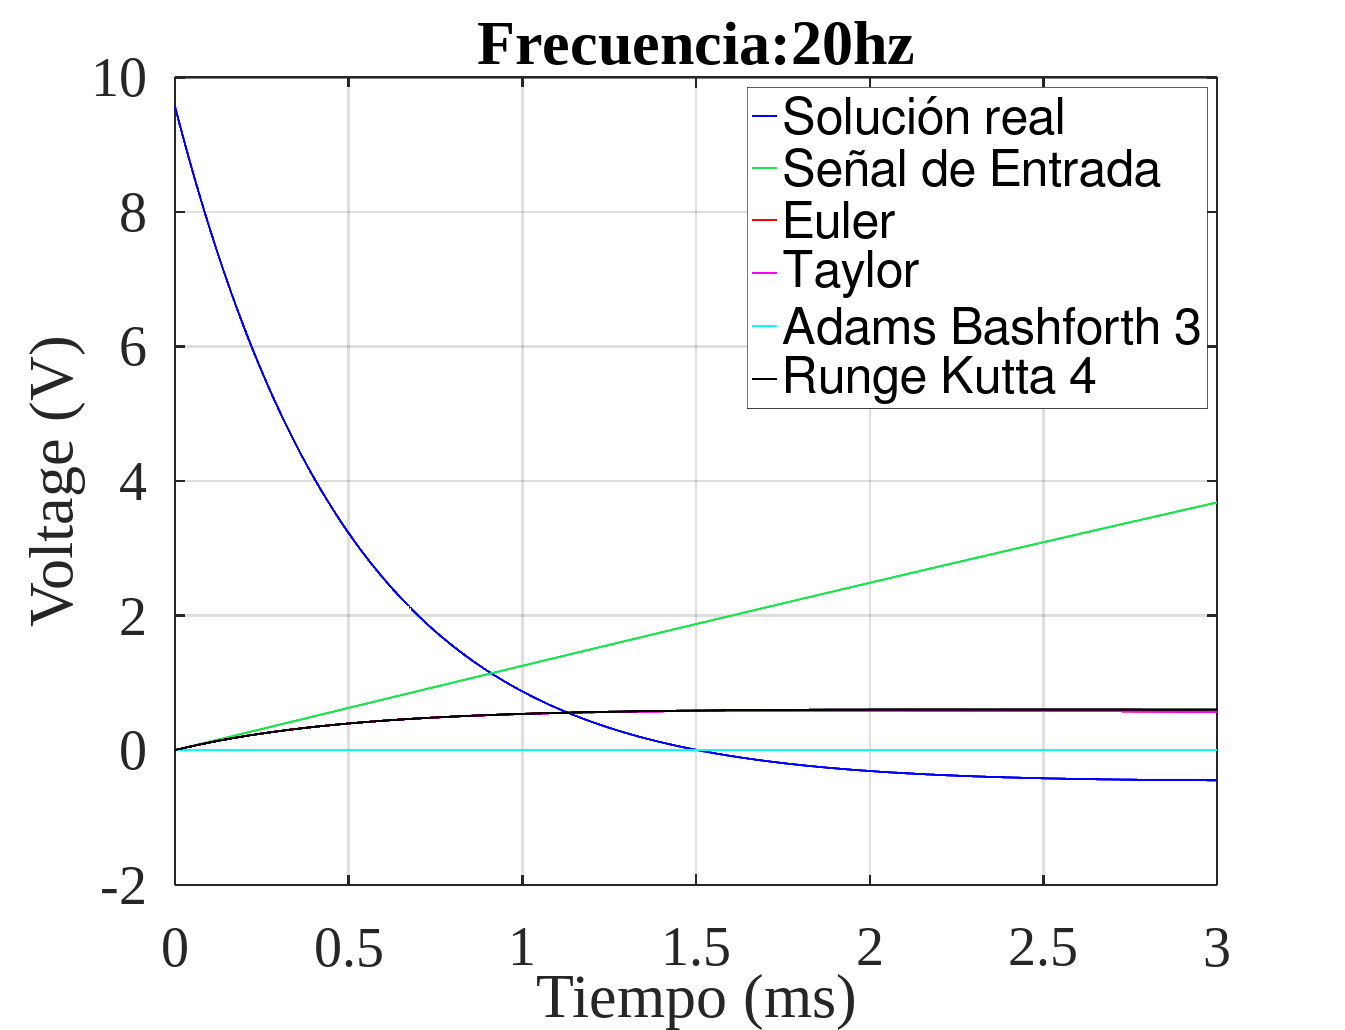
\includegraphics[width=0.43\textwidth]{../plots/ej5/Frecuencia:20hz-ue.png}
\label{fig:fig}
\end{figure}

\begin{figure}[H]
\centering
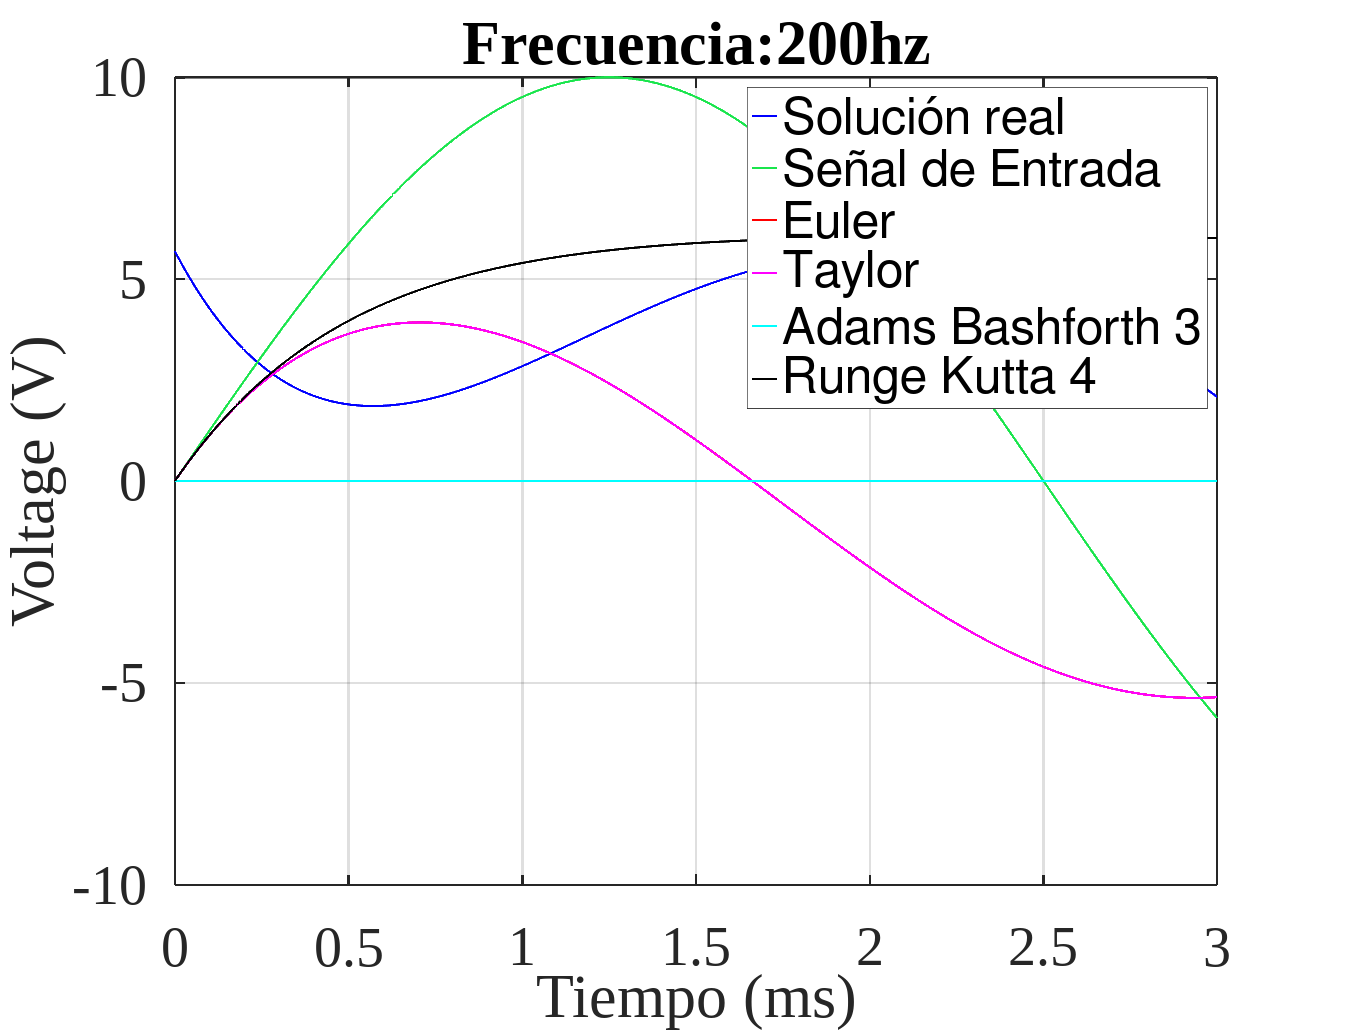
\includegraphics[width=0.43\textwidth]{../plots/ej5/Frecuencia:200hz-ue.png}
\label{fig:fig}
\end{figure}

\begin{figure}[H]
\centering
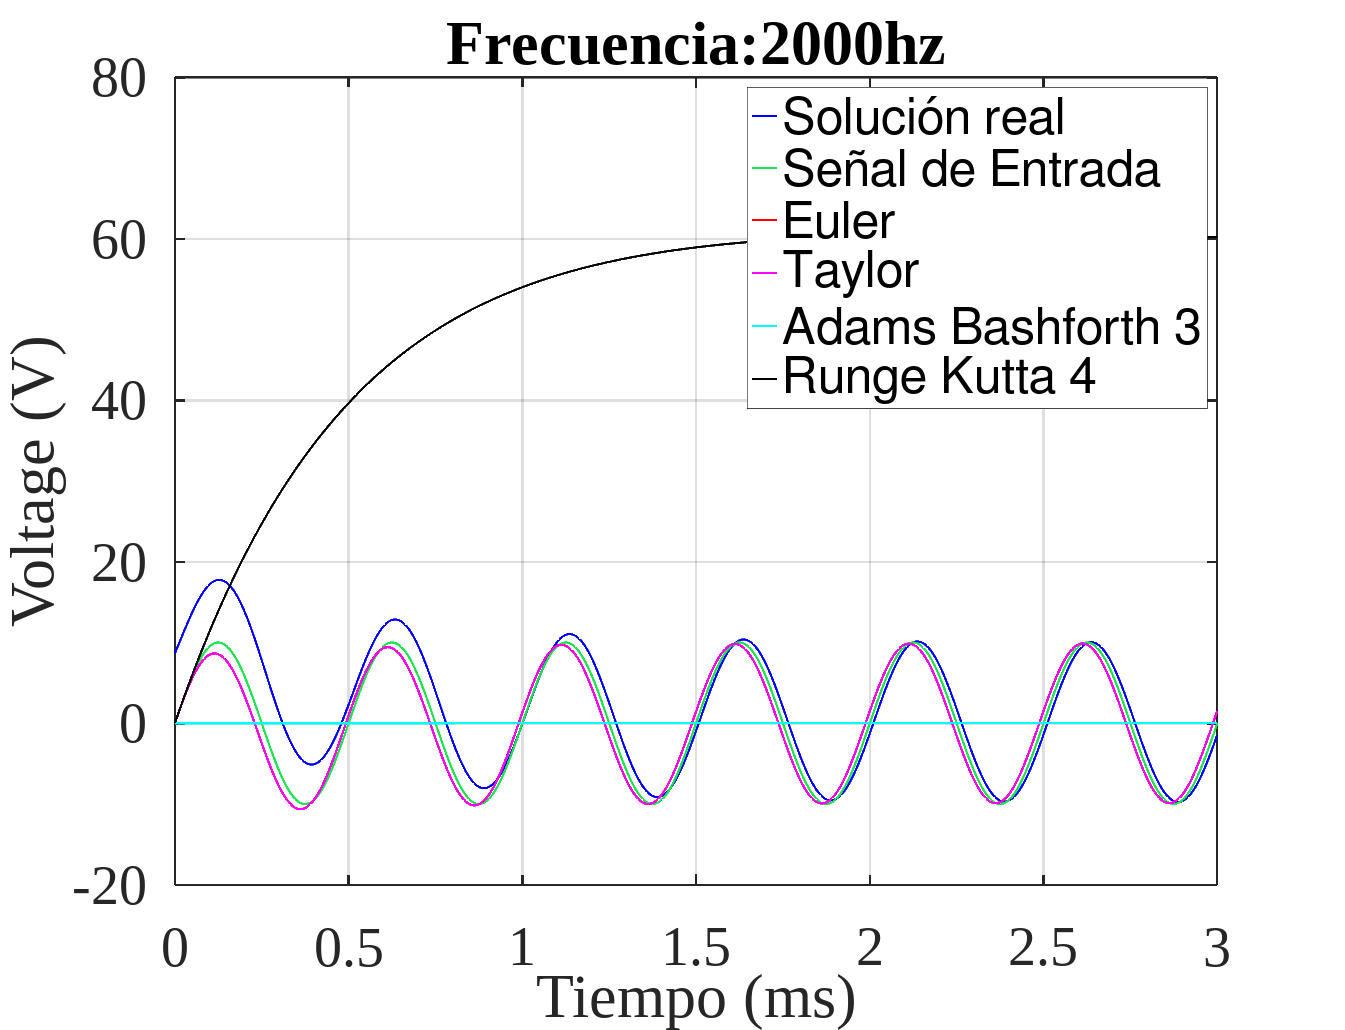
\includegraphics[width=0.43\textwidth]{../plots/ej5/Frecuencia:2000hz-ue.png}
\label{fig:fig}
\end{figure}

\begin{figure}[H]
\centering
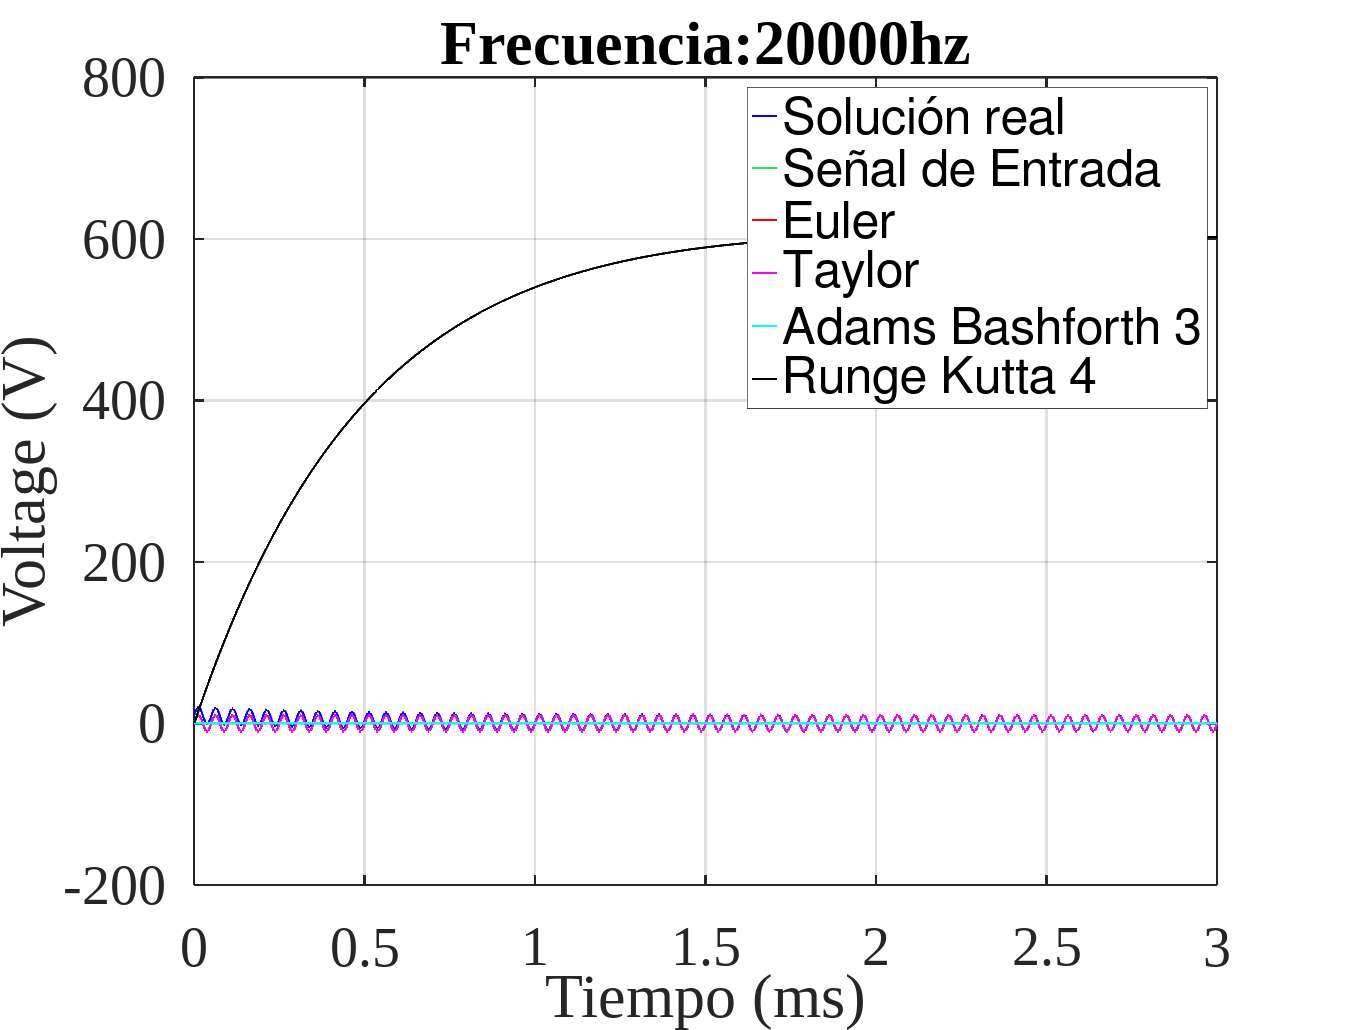
\includegraphics[width=0.43\textwidth]{../plots/ej5/Frecuencia:20000hz-ue.png}
\label{fig:fig}
\end{figure}

Como se observan en estos gr\'aficos efectivamente la señal de salida se ve atenuada (menor voltage) para las frecuencias de entrada bajas, y que como se mencion\'o anteriormente el m\'etodo de Runge Kutta no nos sirve para expresar el comportamiento del circuito, pues diverge. Esto se deduce a partir de que en las frecuencias bajas el voltage m\'aximo que se observa en la salida es cuantitativamente menor y, para frecuencias altas, la señal de salida se comporta pr\'acticamente como la de entrada.
\begin{thebibliography}{99}

\bibitem{c1}	Richard L. Burden, An\'alisis Num\'erico, d\'ecima edici\'on, 2017.
\bibitem{c1}    Steven C. Chapra, Numerical Methods for Engineers, sixth edition, 2010.

\end{thebibliography}

\end{document}
